% -*- Mode: noweb; noweb-default-code-mode: R-mode; -*-
%\SweaveUTF8
\documentclass[11pt]{article}\usepackage[]{graphicx}\usepackage[]{color}
% maxwidth is the original width if it is less than linewidth
% otherwise use linewidth (to make sure the graphics do not exceed the margin)
\makeatletter
\def\maxwidth{ %
  \ifdim\Gin@nat@width>\linewidth
    \linewidth
  \else
    \Gin@nat@width
  \fi
}
\makeatother

\definecolor{fgcolor}{rgb}{0.345, 0.345, 0.345}
\newcommand{\hlnum}[1]{\textcolor[rgb]{0.686,0.059,0.569}{#1}}%
\newcommand{\hlstr}[1]{\textcolor[rgb]{0.192,0.494,0.8}{#1}}%
\newcommand{\hlcom}[1]{\textcolor[rgb]{0.678,0.584,0.686}{\textit{#1}}}%
\newcommand{\hlopt}[1]{\textcolor[rgb]{0,0,0}{#1}}%
\newcommand{\hlstd}[1]{\textcolor[rgb]{0.345,0.345,0.345}{#1}}%
\newcommand{\hlkwa}[1]{\textcolor[rgb]{0.161,0.373,0.58}{\textbf{#1}}}%
\newcommand{\hlkwb}[1]{\textcolor[rgb]{0.69,0.353,0.396}{#1}}%
\newcommand{\hlkwc}[1]{\textcolor[rgb]{0.333,0.667,0.333}{#1}}%
\newcommand{\hlkwd}[1]{\textcolor[rgb]{0.737,0.353,0.396}{\textbf{#1}}}%
\let\hlipl\hlkwb

\usepackage{framed}
\makeatletter
\newenvironment{kframe}{%
 \def\at@end@of@kframe{}%
 \ifinner\ifhmode%
  \def\at@end@of@kframe{\end{minipage}}%
  \begin{minipage}{\columnwidth}%
 \fi\fi%
 \def\FrameCommand##1{\hskip\@totalleftmargin \hskip-\fboxsep
 \colorbox{shadecolor}{##1}\hskip-\fboxsep
     % There is no \\@totalrightmargin, so:
     \hskip-\linewidth \hskip-\@totalleftmargin \hskip\columnwidth}%
 \MakeFramed {\advance\hsize-\width
   \@totalleftmargin\z@ \linewidth\hsize
   \@setminipage}}%
 {\par\unskip\endMakeFramed%
 \at@end@of@kframe}
\makeatother

\definecolor{shadecolor}{rgb}{.97, .97, .97}
\definecolor{messagecolor}{rgb}{0, 0, 0}
\definecolor{warningcolor}{rgb}{1, 0, 1}
\definecolor{errorcolor}{rgb}{1, 0, 0}
\newenvironment{knitrout}{}{} % an empty environment to be redefined in TeX

\usepackage{alltt}
\usepackage{graphicx}
%% \usepackage{Sweave}
\usepackage[utf8]{inputenc}
%% \usepackage{germanU}
%%- \usepackage[noae]{Sweave}
\usepackage[a4paper, text={14.5cm,22cm}]{geometry}
\usepackage{color} %uncomment BF
\usepackage{booktabs} % nice tables with \toprule \middlerule \bottomrule
\usepackage{amsmath} % for align
% \usepackage{wasysym} % for promille sign
% \usepackage{amssymb}
% \usepackage[textfont=it,font=small,labelfont=it]{caption}
\interfootnotelinepenalty=10000 % prevent LaTex from two-sided footnotes
\usepackage{pldescr}
%\VignetteEngine{knitr::knitr}
%\VignetteDepends{plgraphics}
%\VignetteIndexEntry{'plgraphics': A user-oriented collection of graphical R-functions based on the 'pl' concept}

\addtolength{\textwidth}{2.5cm}%%--- 15.0 + 2.5 = 17.5
\addtolength{\oddsidemargin}{-1.04cm}

%% ================================================================
\IfFileExists{upquote.sty}{\usepackage{upquote}}{}
\begin{document}
%% \SweaveOpts{concordance=TRUE,width=9,height=6, echo=false}
\setkeys{Gin}{width=0.9\textwidth}
\baselineskip 15pt
\parskip 10pt

\title{\vspace*{-10mm}
`plgraphics': A user-oriented collection of graphical R-functions based on
 the `pl' concept}
\author{Werner A. Stahel, ETH Zurich}
\maketitle

\begin{abstract}\noindent
The package, \T{plgraphics}, collects enhanced versions of basic plotting
functions. It is based on a paradigm between the basic R graphics elements
and the more computer science oriented ggplot concepts.
The intention is to furnish user-oriented functions that allow efficient
production of useful graphics.
\end{abstract}



\tableofcontents

\pagebreak
\section{Introduction}

The plotting functionality is the historical origin of the R package.
It has been introduced half a century ago and has grown for a while.
For the sake of upward compatibility, it has been essentially unchanged for
several decades. 

New graphical concepts, adjusted to the development of graphical devices
and computer science ideas have been implemented in new packages, 
notably \T{ggplot} ...

The intention of the package \T{plgraphics} is to implement some functions
that provide efficient production of simple to rather sophisticated plots,
but are still based on the core R functionality.
They have been developed over a long time with a focus on allowing 
for readily interpretable graphical diagnostics for regression model
development. 

The general idea is that it should be easy to produce standard plots 
by a simple call like \T{plot(x,y)} or \T{plot(y$\sim$x, data=dd)}, 
as well as enhancing the plot by adding an argument like \T{smooth=TRUE} 
to ask for a smoother or specifying 
a column in the dataset that drives the color or yields labels to mark the
points to be shown. 
Furthermore, the plots should remain useful if there are outliers 
or one of the two
variables is a grouping factor instead of a quantitative variable.

Asking that a basic function provides many variations under the control of
the user means that a large list of arguments must be available.
Some of these variations depend on the taste of the user. 
They can be specified in a kind of ``style list,'' analogous to 
\T{options} and \T{par}, which is called \T{ploptions}.

The package also provides enhanced low level graphical functions
like \T{plpoints}, which extends the functionality of \T{points}.
This leads to a short basic scatterplot function \T{plyx} that can
easily be modified by the user.

This document presents the main features of the package \T{plgraphics}
and explains the concepts behind them. 

The package is available from \T{R-forge}, e.g. by calling\\
\T{install.packages("plgraphics", repos="http://r-forge.r-project.org")}.\\

\section{Scatterplots}

\subsection{The basic scatterplot}
A basic scatterplot is generated by calling \T{plyx}
(plot y on x),
\begin{knitrout}
\definecolor{shadecolor}{rgb}{0.969, 0.969, 0.969}\color{fgcolor}\begin{kframe}
\begin{alltt}
\hlkwd{plyx}\hlstd{(Sepal.Width}\hlopt{~}\hlstd{Sepal.Length,} \hlkwc{data}\hlstd{=iris,} \hlkwc{smooth}\hlstd{=}\hlnum{FALSE}\hlstd{)}
\end{alltt}
\end{kframe}
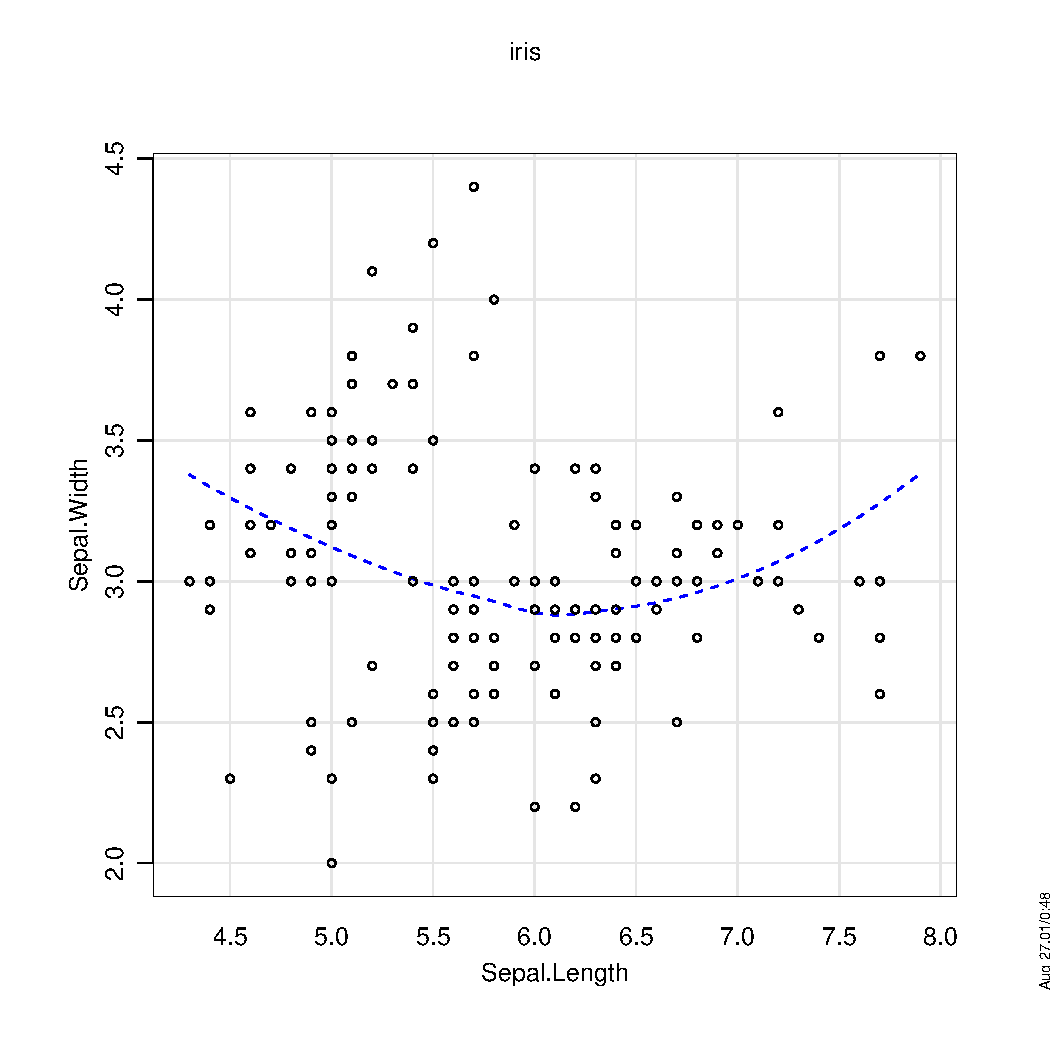
\includegraphics[width=\maxwidth]{figure/plyx-1} 

\end{knitrout}
Clearly, this stongly resembles the result of simply calling \T{plot}, 
except for the thin gridlines and some documentation added by default: 
The name of the dataset is shown as a (sub-) title, and there is a small
text in the lower right corner that shows the date.
%% and a project label that has been set by typing 
%% \T{options(project="pl documentation")}.
Without \T{smooth=FALSE}, a smooth line is added, see below.

More arguments allow to specify many aspects of the plot.
\begin{knitrout}
\definecolor{shadecolor}{rgb}{0.969, 0.969, 0.969}\color{fgcolor}\begin{kframe}
\begin{alltt}
\hlkwd{plyx}\hlstd{(Sepal.Width}\hlopt{~}\hlstd{Sepal.Length,} \hlkwc{data}\hlstd{=iris,}
     \hlkwc{psize}\hlstd{=Petal.Length}\hlopt{^}\hlnum{2}\hlstd{,} \hlkwc{pcol}\hlstd{=Species,} \hlkwc{pch}\hlstd{=Species,} \hlkwc{cex}\hlstd{=}\hlnum{1.3}\hlstd{)}
\end{alltt}
\end{kframe}
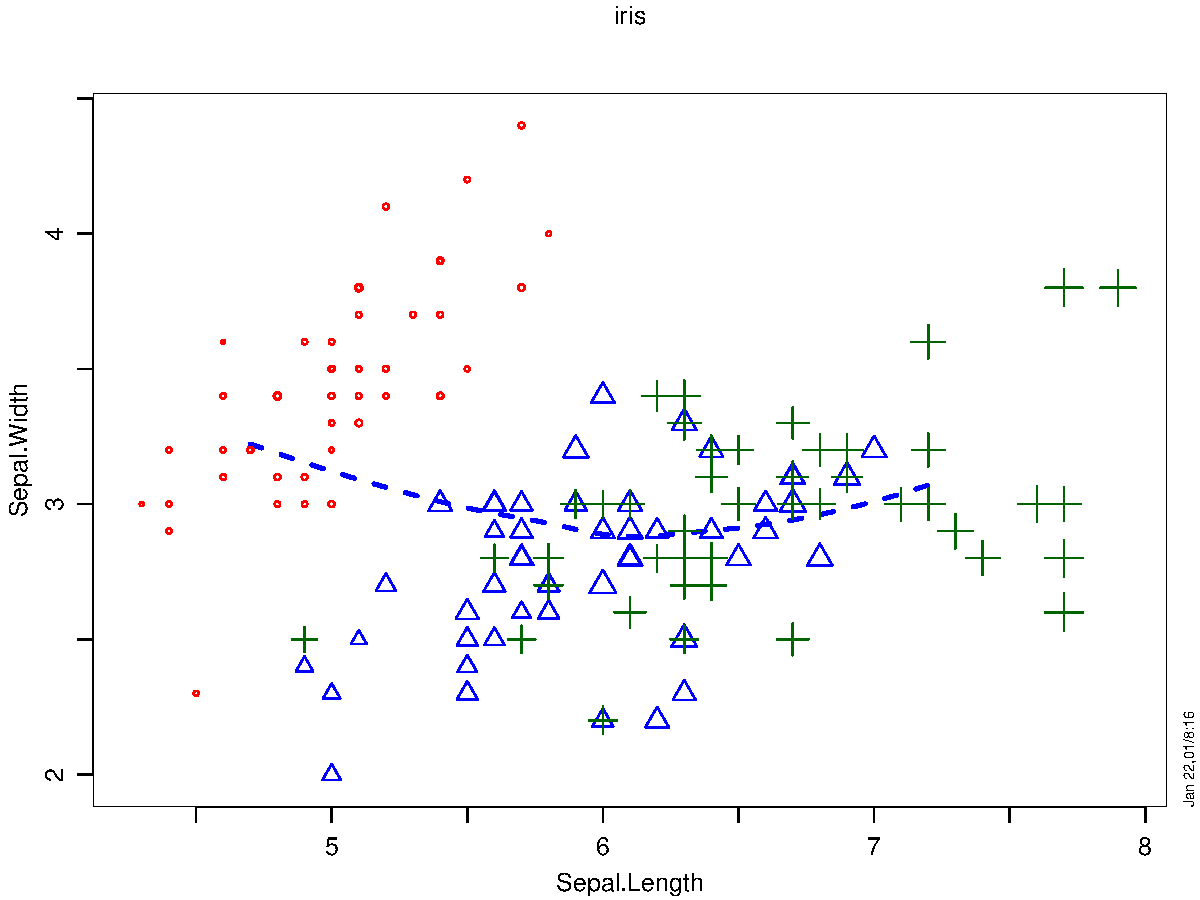
\includegraphics[width=\maxwidth]{figure/plyx_pchar-1} 

\end{knitrout}
The argument \T{psize} sets the size of the plotting symbols
such that their area is proportional to it.
The median size is determined by \T{cex}.
By default, this value adjusts to the number of observations.
\T{pcol} specifies the colors of the symbols.

See \ref{plproperties} for details.

\Tit{Smooth.}
A smooth line fitting the data in the plot is produced if 
\T{smooth=TRUE}, which is the default value. 
The line type, width and color are modified by respective arguments.

Smooths can also be fitted groupwise by specifying \T{smooth.group}.

\begin{knitrout}
\definecolor{shadecolor}{rgb}{0.969, 0.969, 0.969}\color{fgcolor}\begin{kframe}
\begin{alltt}
\hlkwd{plmframes}\hlstd{(}\hlnum{1}\hlstd{,}\hlnum{2}\hlstd{,} \hlkwc{mar}\hlstd{=}\hlkwd{c}\hlstd{(}\hlnum{3}\hlstd{,}\hlnum{3}\hlstd{,}\hlnum{1}\hlstd{,}\hlnum{1}\hlstd{))}
\hlkwd{plyx}\hlstd{(Sepal.Width}\hlopt{~}\hlstd{Sepal.Length,} \hlkwc{data}\hlstd{=iris,} \hlkwc{smooth.col}\hlstd{=}\hlstr{"red"}\hlstd{)}

\hlkwd{plyx}\hlstd{(Sepal.Width}\hlopt{~}\hlstd{Sepal.Length,} \hlkwc{data}\hlstd{=iris,} \hlkwc{smooth.group}\hlstd{=Species,}
     \hlkwc{pcol}\hlstd{=Species)}
\end{alltt}
\end{kframe}
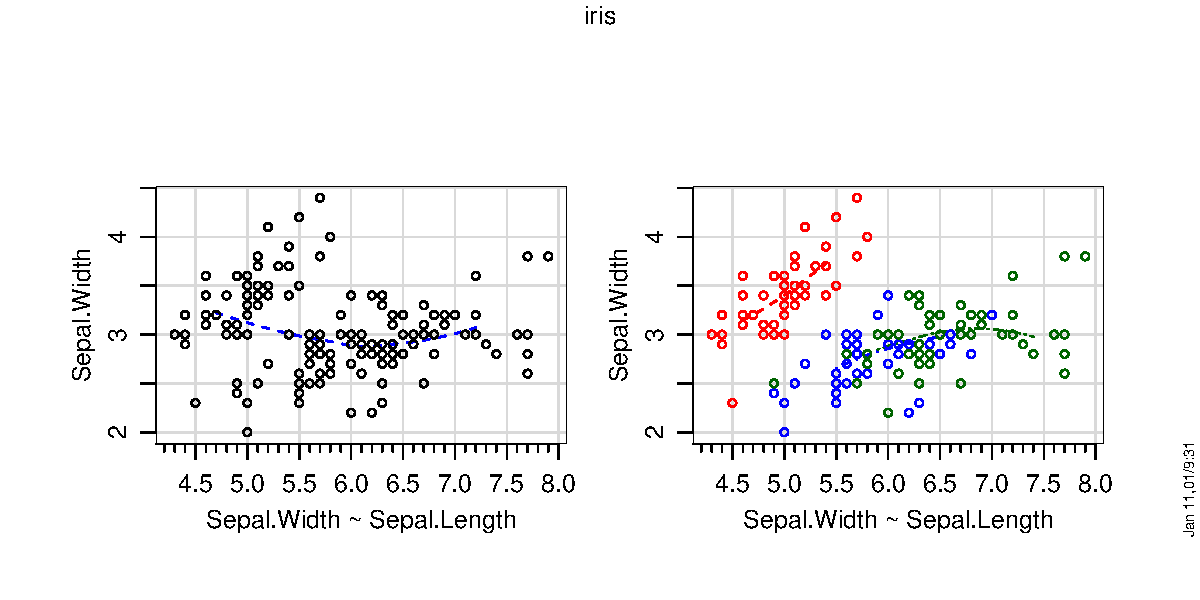
\includegraphics[width=\maxwidth]{figure/plyx_smooth-1} 

\end{knitrout}
Setting \T{pcol=Species} allowed the color of plotting symbols and smooth
lines to be the same.
The call to \T{plmframes} splits the screen essentially like 
\T{par(mfrow=c(1,2))}.

\Tit{Groups.}
If the argument \T{group} is specified, separate plots will be generated
for the different groups, thereby maintaining the plot ranges.

\begin{knitrout}
\definecolor{shadecolor}{rgb}{0.969, 0.969, 0.969}\color{fgcolor}\begin{kframe}
\begin{alltt}
\hlkwd{plmframes}\hlstd{(}\hlnum{1}\hlstd{,}\hlnum{3}\hlstd{)}
\hlkwd{plyx}\hlstd{(Sepal.Width}\hlopt{~}\hlstd{Sepal.Length,} \hlkwc{data}\hlstd{=iris,} \hlkwc{group}\hlstd{=Species)}
\end{alltt}
\end{kframe}
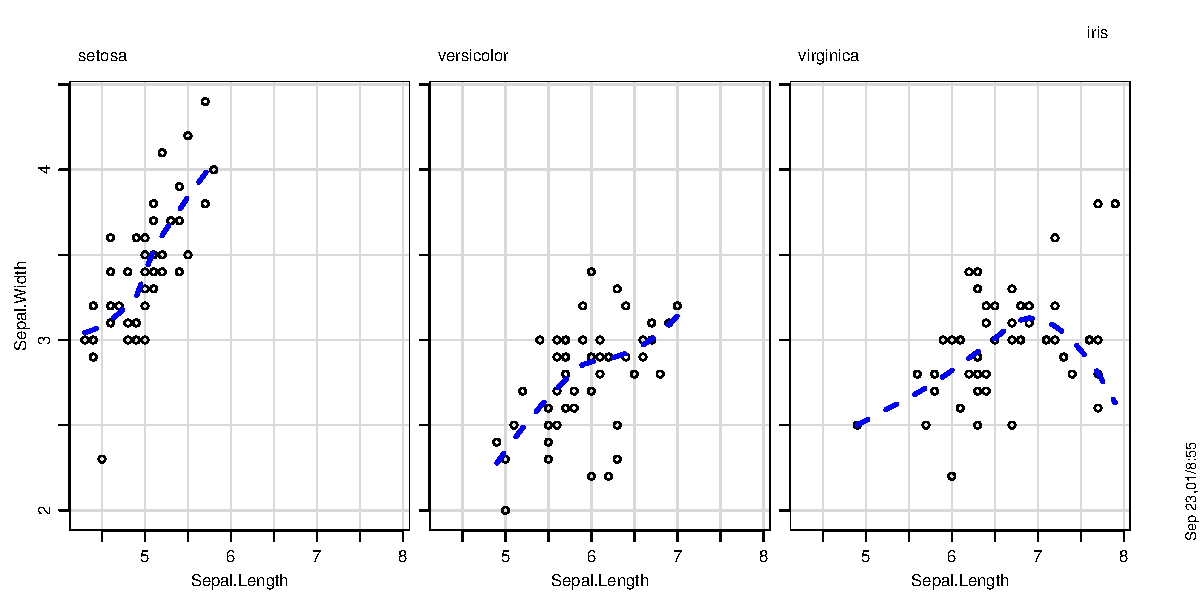
\includegraphics[width=\maxwidth]{figure/plyx_group-1} 

\end{knitrout}

\Tit{Inner range of plots.}
When there are outliers in the data, plots are dominated by their effect of
determining the plotting range. This means that the user who would like to
see more detail about the ``regular'' observations needs to gnerate a new
plot, specifying the limits of the plotting range by \T{xlim} and \T{ylim},
and the outliers will disappear.

In order to avoid the urge for two versions of the plot, an ``inner
plotting range'' is determined, based on robust measures of 
location and scale. Outside this range, there is a plotting margin where
coordinates are transformed with a highly nonlinear function in order to
accomodate all outliers. 
In these margins, the order of coordinates is still maintained, thus
allowing to see which points are further out than others, but quantitative
information is distorted by the transformation.
The figure shows data from the blasting example with an added outlier,
plotted without and with inner plotting limits.

\begin{knitrout}
\definecolor{shadecolor}{rgb}{0.969, 0.969, 0.969}\color{fgcolor}\begin{kframe}
\begin{alltt}
\hlkwd{data}\hlstd{(d.blast)}
\hlstd{dd} \hlkwb{<-} \hlstd{d.blast}
\hlstd{dd}\hlopt{$}\hlstd{distance[}\hlnum{2}\hlstd{]} \hlkwb{<-} \hlnum{200}

\hlkwd{plmframes}\hlstd{(}\hlnum{1}\hlstd{,}\hlnum{3}\hlstd{,} \hlkwc{mar}\hlstd{=}\hlkwd{c}\hlstd{(}\hlnum{3}\hlstd{,}\hlnum{3}\hlstd{,}\hlnum{1}\hlstd{,}\hlnum{1}\hlstd{))}

\hlkwd{plyx}\hlstd{( tremor}\hlopt{~}\hlstd{distance,} \hlkwc{data}\hlstd{=dd,} \hlkwc{innerrange}\hlstd{=}\hlnum{FALSE}\hlstd{)}
\hlkwd{plyx}\hlstd{( tremor}\hlopt{~}\hlstd{distance,} \hlkwc{data}\hlstd{=dd)}
\hlkwd{plyx}\hlstd{( tremor}\hlopt{~}\hlstd{distance,} \hlkwc{data}\hlstd{=dd,} \hlkwc{innerrange.factor}\hlstd{=}\hlnum{5}\hlstd{)}
\end{alltt}
\end{kframe}
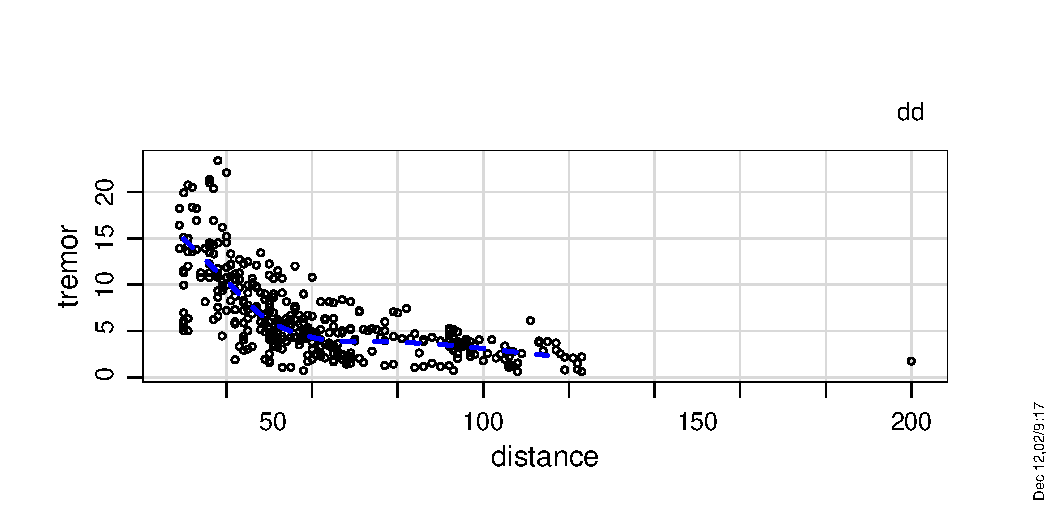
\includegraphics[width=\maxwidth]{figure/innerrange-1} 

\end{knitrout}

If \T{innerrange=TRUE}, which is the default, the \T{plgraphics} functions
will determine an ``inner plotting range'' based on 
the 20\% trimmed mean and a 20\% trimmed scale by default.


%% innerrange
\Detail{The function \T{robrange}, which is called by \T{plinnerrange},
  determines the $\alpha$-trimmed mean with $\alpha=0.2$ as the location 
  and the (one-sided) trimmed mean of the deviations from it. 
  It adjusts this latter mean to obtain an approximately consistent
  estimate of the standard deviation for normal observations. 
  It then calculates the location plus-minus 
  \T{innerrange.factor} times the scale to get a potential inner range.
  The final inner plotting range will be the intersection of this and the
  ordianry range of the values.
}
%% ------------------------------

\subsection{Multiple y and x}
Two or more variables may be given to be plotted on the vertical axis,
in the sense of \T{matplot} of R.
Often, these are parallel time series, and it is convenient to ask for 
lines connecting the points, either \T{type="l"} or \T{type="b"}.
\T{plyx} will choose different scales for the different variables unless
\T{rescale=FALSE}.

\begin{knitrout}
\definecolor{shadecolor}{rgb}{0.969, 0.969, 0.969}\color{fgcolor}\begin{kframe}
\begin{alltt}
\hlkwd{plyx}\hlstd{(}\hlnum{1}\hlopt{:}\hlnum{40}\hlstd{, EuStockMarkets[}\hlnum{1}\hlopt{:}\hlnum{40}\hlstd{,],} \hlkwc{type}\hlstd{=}\hlstr{"b"}\hlstd{,} \hlkwc{smooth.xtrim}\hlstd{=}\hlnum{0.05}\hlstd{)}
\end{alltt}
\end{kframe}
\includegraphics[width=\maxwidth]{figure/plyx-multipley-1} 

\end{knitrout}

The following plot shows a more elaborate example of a time series plot,
see \ref{options.dateaxis} and \ref{options.smooth}
for details about the generation of a time axis and
the additional arguments of \T{plyx}, respectively.

\begin{knitrout}
\definecolor{shadecolor}{rgb}{0.969, 0.969, 0.969}\color{fgcolor}\begin{kframe}
\begin{alltt}
  \hlkwd{data}\hlstd{(d.river)}
  \hlkwd{plyx}\hlstd{(T}\hlopt{+}\hlstd{O2}\hlopt{+}\hlstd{ra}\hlopt{+}\hlstd{Q}\hlopt{~}\hlstd{date,} \hlkwc{data}\hlstd{=d.river,}
       \hlkwc{subset}\hlstd{=date}\hlopt{<}\hlkwd{as.Date}\hlstd{(}\hlstr{"2010-03-31"}\hlstd{)}\hlopt{&}\hlstd{hour}\hlopt{==}\hlnum{14}\hlstd{,}
       \hlkwc{smooth.par}\hlstd{=}\hlnum{0.5}\hlstd{,} \hlkwc{smooth.xtrim}\hlstd{=}\hlnum{0.03}\hlstd{,} \hlkwc{smooth.lty}\hlstd{=}\hlnum{1}\hlstd{,} \hlkwc{sub}\hlstd{=}\hlstr{"river data"}\hlstd{)}
\end{alltt}
\end{kframe}
\includegraphics[width=\maxwidth]{figure/plyx-time-1} 

\end{knitrout}

If multiple x variables are given, a separate plot is drawn for each of them.
\begin{knitrout}
\definecolor{shadecolor}{rgb}{0.969, 0.969, 0.969}\color{fgcolor}\begin{kframe}
\begin{alltt}
\hlkwd{plmframes}\hlstd{(}\hlnum{1}\hlstd{,}\hlnum{2}\hlstd{,} \hlkwc{mar}\hlstd{=}\hlkwd{c}\hlstd{(}\hlnum{3}\hlstd{,}\hlnum{3}\hlstd{,}\hlnum{3}\hlstd{,}\hlnum{1}\hlstd{))}
\hlkwd{plyx}\hlstd{(Sepal.Length}\hlopt{~}\hlstd{Petal.Length}\hlopt{+}\hlstd{Petal.Width,} \hlkwc{data}\hlstd{=iris,}
     \hlkwc{smooth.group}\hlstd{=Species,} \hlkwc{pcol}\hlstd{=Species)}
\end{alltt}
\end{kframe}
\includegraphics[width=\maxwidth]{figure/plyx-multiplex-1} 

\end{knitrout}
%% \label{multiplex}

%%- \subsection{Groups}
%%- The argument \T{group} is used to generate multiple plots, one for each 
%%- factor level, using the same plotting scales and ranges.
%%- <plyx_group, fig_height=4>
%%- plmframes(1,3, mar=c(1,1,1,1))
%%- plyx(Sepal.Width~Sepal.Length, data=iris, group=Species)
%%- @ 

\Tit{Raw or transformed variables?}
Simple formulas just include names of variables on both sides of the $\sim$
symbol, separated by ``+'' if there are more than one. 
More advanced formulas consist of terms.
(Interaction terms act as two separate terms here.)
The user can choose if he or she wants to plot the terms or the variables
that are involved. 
The most common terms beyond raw variables are transformed variables.
If the argument \T{transformed} is \T{TRUE}, the terms will be used as
plotting variables (horizontal or vertical). 
Otherwise, the plotting variables are obained by applying \T{all.vars} to
both sides of the formula.

\begin{knitrout}
\definecolor{shadecolor}{rgb}{0.969, 0.969, 0.969}\color{fgcolor}\begin{kframe}
\begin{alltt}
  \hlkwd{plyx}\hlstd{(}\hlkwd{log10}\hlstd{(Sepal.Length)} \hlopt{~} \hlkwd{log10}\hlstd{(Petal.Length}\hlopt{*}\hlstd{Petal.Width),}
       \hlkwc{data}\hlstd{=iris,} \hlkwc{smooth.group}\hlstd{=Species,} \hlkwc{pcol}\hlstd{=Species,} \hlkwc{transformed}\hlstd{=}\hlnum{TRUE}\hlstd{)}
\end{alltt}
\end{kframe}
\includegraphics[width=\maxwidth]{figure/pluntransformed-1} 

\end{knitrout}

Setting \T{transformed = FALSE} produces the same figure as
\ref{multiplex}

%%- <<pltransformed, fig.height=4>>=
%%-   plmframes(1,2)
%%-   plyx(log10(Sepal.Length) ~ log10(Petal.Length*Petal.Width), 
%%-        data=iris, smooth.group=Species, pcol=Species, transformed=FALSE)
%%- @ 

\subsection{Nonlinear plotting scales}

In basic R graphics, ``log scale'' may be selected by specifying 
\T{log="y"} (or \T{="x"} or \T{="xy"}). \Hneed{35mm}
\T{plgraphics}\ allows for any monotone transformation.
For example, the arc sine transformation \Hneed{60mm}
$\mbox{asinp}\fn x = \mbox{arcsin}\big(\sqrt{x/100}\big) /
\mbox{arcsin}\fn{1}$ \ 
is recommended as a ``first aid transformation'' for percentages.
Rather than plotting the transformed variable, the \T{plgraphics}
functions offer the argument \T{plscale}, which leads to using the 
function \T{plscale} and shows the transformed data with tick marks
refelcting the original scale (as \T{log="y"} would do it for basic R).
\label{intro.plscale}

\begin{knitrout}
\definecolor{shadecolor}{rgb}{0.969, 0.969, 0.969}\color{fgcolor}\begin{kframe}
\begin{alltt}
  \hlkwd{data}\hlstd{(d.babysurvGr)}
  \hlkwd{showd}\hlstd{(d.babysurvGr)}
\end{alltt}
\begin{verbatim}
## dim:  10 4 
##      n Survival.0 Survival.1 Weight
## 1   10         10          0    550
## 2   14         12          2    650
## 3   27         18          9    750
## ...                                
## 5   32          9         23    950
## 6   28          7         21   1050
## 8   26          7         19   1250
## 10  32          3         29   1450
\end{verbatim}
\begin{alltt}
  \hlkwd{plyx}\hlstd{(}\hlkwd{I}\hlstd{(}\hlnum{100}\hlopt{*}\hlstd{Survival.1}\hlopt{/}\hlstd{n)} \hlopt{~} \hlstd{Weight,} \hlkwc{data}\hlstd{=d.babysurvGr,} \hlkwc{plscale}\hlstd{=}\hlkwd{c}\hlstd{(}\hlstr{"log"}\hlstd{,}\hlstr{"asinp"}\hlstd{))}
\end{alltt}
\end{kframe}
\includegraphics[width=\maxwidth]{figure/plyx-plscale-1} 

\end{knitrout}

\subsection{Marking extreme points}

Extreme points are often of interest. They can easily be identified if they 
are labelled. This is achieved by setting the argument \T{markextremes}.

\begin{knitrout}
\definecolor{shadecolor}{rgb}{0.969, 0.969, 0.969}\color{fgcolor}\begin{kframe}
\begin{alltt}
\hlkwd{plmframes}\hlstd{(}\hlnum{1}\hlstd{,}\hlnum{2}\hlstd{,} \hlkwc{mar}\hlstd{=}\hlkwd{c}\hlstd{(}\hlnum{3}\hlstd{,}\hlnum{3}\hlstd{,}\hlnum{3}\hlstd{,}\hlnum{1}\hlstd{))}

\hlkwd{plyx}\hlstd{(Sepal.Width}\hlopt{~}\hlstd{Sepal.Length,} \hlkwc{data}\hlstd{=iris[}\hlnum{1}\hlopt{:}\hlnum{50}\hlstd{,],} \hlkwc{smooth}\hlstd{=F,}
     \hlkwc{markextremes}\hlstd{=}\hlnum{0.1}\hlstd{,} \hlkwc{cex}\hlstd{=}\hlnum{0.7}\hlstd{)}
\hlcom{## different proportions marked in different margins:}
\hlkwd{plyx}\hlstd{(Sepal.Width}\hlopt{~}\hlstd{Sepal.Length,} \hlkwc{data}\hlstd{=iris[}\hlnum{1}\hlopt{:}\hlnum{50}\hlstd{,],} \hlkwc{smooth}\hlstd{=F,}
     \hlkwc{markextremes}\hlstd{=}\hlkwd{list}\hlstd{(}\hlnum{0}\hlstd{,}\hlkwd{c}\hlstd{(}\hlnum{0.02}\hlstd{,}\hlnum{0.2}\hlstd{)),} \hlkwc{cex}\hlstd{=}\hlnum{0.7}\hlstd{)}
\end{alltt}
\end{kframe}
\includegraphics[width=\maxwidth]{figure/markextremes-1} 

\end{knitrout}
The default value of \T{markextremes} is 0 for \T{plyx}.
If the argument is \T{NA}, it depends on the number of 
observations: It is $1/(2\sqrt{n})$. 

\subsection{The Multibox Plot for factors}
If the x variable is a factor, R's generic plot function for formula objects
draws box plots.
When there are many observations per group, a box plot constitutes a 
very rough image of the distributeion.
The ``multibox plot'' is a refinement that shows the distribution in more
detail. 

The idea is to combine the virtues of the box plot, which is based on the
quartiles, with those of a histogram that depicts the density of the
distribution. 
Essentially, a histogram is drawn using quantiles as class limits.
(Since raw quantiles may be poor characterizations for discrete data,
``interpolated quantiles'' are used as class limits.)

The number of quantiles -- or the number of classes -- used should be
adapted to the number of observations to be represented.
For moderate sample sizes, ``octiles'' appear suitable.

The multibox plot can be called directly.
\begin{knitrout}
\definecolor{shadecolor}{rgb}{0.969, 0.969, 0.969}\color{fgcolor}\begin{kframe}
\begin{alltt}
\hlkwd{plmframes}\hlstd{()}  \hlcom{## reset to just 1 figure per plot}
\hlcom{## plyx(Sepal.Width~Species, data=iris)  ## -- or --}
\hlkwd{plmboxes}\hlstd{(Petal.Length}\hlopt{~}\hlstd{Species,} \hlkwc{data}\hlstd{=iris)}
\end{alltt}
\end{kframe}
\includegraphics[width=\maxwidth]{figure/mboxes-1} 

\end{knitrout}

The multiboxes %in Figure \ref{fig:mboxes} 
resemble a well-known kind of
presentation of age distributions. Often, these displays are asymmetric,
showing the age distribution of the two genders on the two sides.
In much the same way, asymmetric multibox plots can be drawn to visualize
the relationship of the continuous variable with any binary variable.
% Figure \ref{fig:mboxes2} shows the distribution of
%%-   Target variable \T{tremor} related to factor{location} and binary variable
%%-   \T{charge>5}
\begin{knitrout}
\definecolor{shadecolor}{rgb}{0.969, 0.969, 0.969}\color{fgcolor}\begin{kframe}
\begin{alltt}
\hlkwd{data}\hlstd{(d.blast)}
\hlkwd{plmboxes}\hlstd{(tremor}\hlopt{~}\hlstd{location}\hlopt{+}\hlkwd{I}\hlstd{(charge}\hlopt{>}\hlnum{5}\hlstd{),} \hlkwc{data}\hlstd{=d.blast)}
\end{alltt}
\end{kframe}
\includegraphics[width=\maxwidth]{figure/mboxes2-1} 

\end{knitrout}

\subsection{Censored data}
Censored data is shown with special symbols, determined by the ploption
\linebreak[3]
\T{censored.pch}. The default for this option contains 8 elements
corresponding to the combined cases of no, right and left censoring of 
the x and y variables.

\begin{knitrout}
\definecolor{shadecolor}{rgb}{0.969, 0.969, 0.969}\color{fgcolor}\begin{kframe}
\begin{alltt}
\hlkwd{require}\hlstd{(}\hlstr{"survival"}\hlstd{)}
\hlkwd{data}\hlstd{(lung,} \hlkwc{package}\hlstd{=}\hlstr{"survival"}\hlstd{)}
\hlkwd{plmframes}\hlstd{(}\hlnum{1}\hlstd{,}\hlnum{2}\hlstd{,}\hlkwc{mar}\hlstd{=}\hlkwd{c}\hlstd{(}\hlnum{3}\hlstd{,}\hlnum{3}\hlstd{,}\hlnum{1}\hlstd{,}\hlnum{1}\hlstd{))}
\hlkwd{plyx}\hlstd{(}\hlkwd{Surv}\hlstd{(time,status)} \hlopt{~} \hlstd{age}\hlopt{+}\hlstd{wt.loss,} \hlkwc{data}\hlstd{=lung,} \hlkwc{pcol}\hlstd{=sex)}
\end{alltt}
\end{kframe}
\includegraphics[width=\maxwidth]{figure/censored-1} 

\end{knitrout}


\section{Scatterplot matrices}
\subsection{plmatrix}
The common type of catterplot matrices are produced by the \T{pairs} function 
in basic R. The function \T{plmatrix} does a similar job.

\begin{knitrout}
\definecolor{shadecolor}{rgb}{0.969, 0.969, 0.969}\color{fgcolor}\begin{kframe}
\begin{alltt}
\hlkwd{plmatrix}\hlstd{(iris,} \hlkwc{smooth.group}\hlstd{=Species,} \hlkwc{pcol}\hlstd{=Species)}
\end{alltt}
\end{kframe}
\includegraphics[width=\maxwidth]{figure/plmatrix-1} 
\begin{kframe}\begin{alltt}
\hlkwd{plmatrix}\hlstd{(}\hlopt{~}\hlstd{Petal.Length}\hlopt{+}\hlstd{Petal.Width,} \hlopt{~}\hlstd{Sepal.Length}\hlopt{+}\hlstd{Sepal.Width,} \hlkwc{data}\hlstd{=iris,}
         \hlkwc{smooth.group}\hlstd{=Species,} \hlkwc{pcol}\hlstd{=Species)}
\end{alltt}
\end{kframe}
\includegraphics[width=\maxwidth]{figure/plmatrix-2} 

\end{knitrout}

The second call to \T{plmatrix} shows that different variables can be
selected for the horizontal and vertical axes. 

If \T{plmatrix} is called for a large dataset, with more than 8 variables, 
say, then it splits the scatterplot matrix into parts that appear on
separate pages in order to avoid that the panels become too small.
The number of panels to be shown in either direction can be set by 
arguments \T{nrow} and \T{ncol}. 
Otherwise, the function will determine suitable numbers 
if the total number of panels exceeds the threshold set in 
\T{ploptions("mfgtotal")}. The default is 30.

\subsection{Conditional plots}
A second handsome funtion in basic graphics that produces a ``matrix''
of scatterplots is the \T{coplot}. 
Each panel is the scatterplot of a pair \T{x} and \T{y} of variables,
where only a subset of points is shown, and the subset is defined
by the intersection of subsets of two variables, the ``conditioning''
variables. The panels are arranged in the natural way to form
a matrix of scatterplots.
The plgrahics version of \T{coplot} is called \T{plcond}.

\begin{knitrout}
\definecolor{shadecolor}{rgb}{0.969, 0.969, 0.969}\color{fgcolor}\begin{kframe}
\begin{alltt}
\hlkwd{plcond}\hlstd{(Sepal.Width}\hlopt{~}\hlstd{Sepal.Length,} \hlkwc{data}\hlstd{=iris,} \hlkwc{condvar}\hlstd{=}\hlopt{~}\hlstd{Species}\hlopt{+}\hlstd{Petal.Length)}
\end{alltt}
\end{kframe}
\includegraphics[width=\maxwidth]{figure/plcond-1} 

\end{knitrout}
The conditioning variables may be factors or numerical variables.
In the latter case, the (robust) range of the variable is partitioned
in a number of equally long intervals. 
%% (The number is given by \T{ploptions("plcond.nintervals")}.)
Each panel then shows the points in the interval in their ordinary appearance,
and, in addition, some points of the neighoring intervals, with reduced size
%% (\T{ploptions("plcond.cex")}) 
and paled color. The color is changed to standard colors indicating whether 
the point's conditioning variable(s) is (are) below or above the interval.
All these features are controled by pl options.

In the expamle, the panel for species setosa and \T{Petal.Length} between
\T{2.18} and \T{3.36} only contains points from the neighoring interval
below, and they are all colored in varying shades of blue, the paling
depending on their distance from the lower limit \T{2.18}.
Similarly, for species virginica, the middle interval contains only one 
point, and the panel noly shows several points that properly contain to the
interval above, in shades of purple.

If only one variable is used for conditioning, the function can also 
be used. It is then an alternative to using \T{plyx} with 
a \T{group} variable.

%% ===========================================================================
\section{Regression diagnostic plots}
Graphical regression diagnostics are the essential tools for developing
adequate models in many statistical problems.
The primary purpose of developing \T{plgraphics} has been to improve
regression diagnostic plots.
The features are obtained by using \T{plregr}.

\subsection{The basic diagnostic plots}
When R objects obtained from fitting a model are fed into R's \T{plot}
function, some fundamental diagnostic plots appear. 
The figure shows the versions of these displays obtained by \T{plregr}
in the case of an ordinary regression.

\begin{knitrout}
\definecolor{shadecolor}{rgb}{0.969, 0.969, 0.969}\color{fgcolor}\begin{kframe}
\begin{alltt}
\hlkwd{data}\hlstd{(d.blast)}
\hlstd{r.blast} \hlkwb{<-}
  \hlkwd{lm}\hlstd{(}\hlkwd{logst}\hlstd{(tremor)}\hlopt{~}\hlstd{location}\hlopt{+}\hlkwd{log10}\hlstd{(distance)}\hlopt{+}\hlkwd{log10}\hlstd{(charge),} \hlkwc{data}\hlstd{=d.blast)}
\hlkwd{plregr}\hlstd{(r.blast,} \hlkwc{xvar}\hlstd{=}\hlnum{FALSE}\hlstd{)}
\end{alltt}
\end{kframe}
\includegraphics[width=\maxwidth]{figure/plotregr-1} 

\end{knitrout}
Before we describe the plots in some detail, let us first explain  
principles guiding the design of diagnostics.
\begin{itemize}
\item
Each diagnostic (plot) should be specific for a well-identified potential 
deficiency of the model.
\item
Plots are selectively shown in accordance with the type of model that has 
been fitted. For example, a normal plot is only shown if the model assumes
a normal distribution of the random error.
\item
Most importantly, residuals are plotted against explanatory variables.
This can also be achieved by calling \T{termplot} for other fit objects,  
but experience shows that this is often neglected by average users.
\item
Residuals can be plotted easily against the index (sequence number) 
of the observation (by setting \T{sequence=TRUE}), 
since this may show trends or correlations of errors in time --
if the sequence reflects time.
\item
The plots are augmented by a smooth line fitted to them -- which is also
available in the classical R functions -- and two additional smooth lines
that allow to judge the scale dependence on the variable shown.
In addition, simulated smooths are added in order to assess an informal 
``significance'' of curvature in the smooth of the data. 
Furthermore, a reference line is given, which helps finding
an appropriate modification of the model if significant curvature is
found. 
\item
Finally, plotting methods are defined for models for which no useful 
methods are available in the basic R packages, notably ordered response
regression and censored responses.
\end{itemize}

\Detail{
  The \t{plotselect} argument is used to modify the default selection and
  to indicate if a smooth should be shown.
  For example, \T{plregr(rr, plotselect=list(yfit=2, qq=0))}
  The plots of residuals against input variables can be suppressed
  by setting the argument \T{xvar=FALSE}.
}

\Detail{
  \T{plregr} saves space around the panels: it reduces 
  \T{ploptions("mar")[3]} by 1.5 (but not lower than 0.5).
  Use \T{mar=c(...)} with a correspondingly larger \T{mar[3]} element if desired.
}

Let us now describe the panels shown above in some detail.

\Tit{Residuals against fit, Tukey-Anscombe plot.}
The plot of residuals against fitted values is the most important
diagnostic tool to assesss the validity of model assumptions.
It allows for detecting deviations from linearity, homoscedasticity,
symmetry and normal distribution of the random deviations.

By default, the scatterplot of residuals against fitted values shows
the points with the feature of outlier margins and marking of extremes in
the residual direction. It adds a smooth line to show deviations from
the linearity assumption. Another 19 smooth lines are shown to 
mimik the variability of this smooth line under the hypothesis that the
model is correct.

If there is curvature, one remedy may be to transform the response
variable. This can help only if the relation between fitted and
response values is monotone -- otherwise, quadratic terms are the
most straightforward modification of the model.
Monotonicity is easy to see if the response is plotted on the vertical
axis instead of the residuals.
This display can also be requested from \T{plot.regr}
(by setting \T{plotselect=c(yfit=3)}).

In order to avoid the necessity to either call \T{plot} again or to 
ask for the plot of response against fitted values routinely,
a \ul{reference line} (green dot-dashed line in the Figure)
is shown in the Tukey-Anscombe plot.
It connects points with equal response values. Since the response can be
determined by adding the two coordinates of the plot -- 
fitted plus residual -- lines of equal response values have slope -1.
The reference line shown is such a line, the one going through the center
of the points in the plot.
If the smooth never gets steeper than the reference line, then the
suggested relation between fitted and response values is monotone, 
and a transformation of the response may remove the non-linearity.

One might argue that a plot of the response on the fit is more
straightforwardly interpreted than the Tukey-Anscombe plot with the
reference line. We think that the Tukey-Anscombe plot can show the
deviations from model assumptions more clearly and should therefore be
preferred, and that the reference line, after a short learning period, will
be easy enough to work with and helps avoiding an additional display. 
Of course, some users may disagree.
%%- 
%%- 
%%- It also adds a reference line indicating the direction of constant observed
%%- response values $Y$. This helps to see whether a transformation of $Y$
%%- could help to avoid any significant curvature.

\Detail{The smoother used by default to generate the smooth lines in the
  plot is \code{\link{loess}(..., span=smooth.par, iter=smooth.iter)},
  where \code{smooth.par} and \code{smooth.iter} are given in 
  \code{ploptions} and the default \code{smooth.par} adapts to the number
  of observations by calling the function \T{smoothpar}.
  If the response of the model is a count (binary-binomial, Poisson with a
  low maximal count, or of class \code{polr}), the non-robust version is 
  called by setting \code{iter} to 0 and the \code{family} argument to 
  \code{gaussian}.
  Otherwise, \code{loess} produces a robust smoother.
}

\Detail{
  \textbf{Smooth band.} \ 
  As mentioned above, in addition to a smooth line fitted to the points,
  a ``low'' and a ``high'' smooth line are shown (unless suppressed).
  They are obtained as follows: Residuals are calculated as the diference
  between the observations and the respective smoothed values $\wh s_i$.
  Then a smooth is calculated for the square roots of the positive residuals,
  and the squared fitted values are added to the $\wh s_i$.
  (The transformation by square roots makes the distribution of the residuals 
  more symmetric.)
  This defines the ``high'' smooth line. 
  The construction of the ``low'' one is analogous.
}  

\Tit{Absolute residuals against fit.}
As a second diagram (often below the first one), the plot of 
absolute residuals against fitted values is shown.
It is intended to detect heteroscedasticity, more precisely,
variances of the random deviations that depend on the expected value
of the response.

Note that the ``absolute residuals'' shown in this plot are not the 
absolute values of the residuals used in the first plot. 
They differ in two ways:
\Itm
They are standardized to have the same variances.
If there are weights of observations (argument \T{weights} in the call to
the fitting function), these are taken as inverse relative variances of
the random errors.
\Itm
By default, they are modified because in the following way.
Note first that the plot should show any dependence of the scale of the
random errors on the model value.
If the plot of residuals against fit shows a clear curvature, the
residuals do not show only the random errors but also the bias of the
regression function, which should be best approximated by the smooth line
in that first plot. Therefore, the residuals from the smooth line are 
used in the plot of absolute residuals against fit.
Additionally, they are standardized using the same factor that is commonly
used for standardizing the ordinary residuals.

\Detail{Basic R's plot method for \T{lm} models (and related ones)
  shows the square root of the absolute residuals.
  They are more symmetrically distributed and therefore more suitable
  for calculating a smooth. 
  \T{plregr} also uses these transformed values for generating the smooth,
  but still shows the absolute residuals and the smoothing line in the
  original scale, since this version is easier to understand.
}

%% censored: no intervals

\Tit{QQ-plot.}
The next plot is the normal quantile-quantile plot. It is only shown if the
residuals are expected to follow a normal distribution.
(QQ-plots for other distributions are planned.)
The standardized residuals are used since a qq-plot for observations with 
different scales does not make sense.

\Tit{Residuals against leverage.}
The influence of individual observations on the results of fitting the model
is measured by the quantities produced by the function \T{influence}.
The most important measures are functions of the residuals and the 
leverage values, often denoted as $h_i$, which are proportional to
Mahalanobis distances from the center of the design based on the 
(formal) covariance matrix of the design.
Therefore, a plot of residuals against leverages should reveal the overly
influential observations.

The leverage plot of \T{plregr} uses \emph{standardized} residuals
in contrast to R's standard leverage plot shown by \T{plot}.
In the case of weighted observations, ``de-weighted'' leverages,
\[
  h_i\sups{dw} = h_i/w_i = \vc x_i\tr (\mx X\tr \mx W \mx X)\inv \vc x_i
\]
are used, but weights are shown by the symbol's sizes.
This version maintains the idea that leverages should be proportional to 
Mahalanobis distances.

\Detail{
  The plot also shows contour lines of constant Cook's distance,
  defined as
\[
  D\sups C_i = \frac{r_i^2}{p\wh\sigma^2}\cdot\frac{h_i}{(1-h_i)^2}
    = {\textstyle 1\over p} \; r_i^{*2} \frac{h_i}{1-h_i}
\;,
\]
where $r_i^*$ denotes the standardized residual.
  Since the mean of $h_i$ is $1/p$, an observation with this leverage
  and a standardized residual of $1$ has $D\sups C=1\big/(p-1)$.
  Contour lines are drawn for $D_i\sups C=\pm c^2\big/(p-1)$, where $c$ is given 
  by \T{ploptions("cookdistlines")}.
  Note that this is different from standard R.
}

%% !!! verschieben?
In several non-Gaussian models, the estimator can be regarded as a weighted
Least Squares estimator with suitable weights. 
Therefore, the weighted version of the leverage plot is produced for such
models. 

\Tit{Weights}
If weights are given by the user, they should usually reflect different
variances of the random errors $E_i$, and the residuals, multiplied by the
square root of the weights, should have constant variance.
The standardized absolute residuals are therefore plotted against the weights.
If the size of these residuals is not constant but depends on the weight, 
the rule or weighting function should be revised.

If weights are given, they are also used as the sizes of the plotting
symbols (circles) in other plots.

%% =================================

The argument \T{xvar=FALSE} in the statement generating the last plot
indicates that by default, \T{plregr} 
shows more diagrams: The plots of residuals against input variables.

The diagrams shown by \T{plregr} and their sequence are determined by
the argument \T{plotselect}, see \T{?plregr} for details.

\subsection{Residuals against input variables}
Since the ``x'' variables in a regression model cannot always be
interpreted as \emph{explaining} the variability of the response $Y$,
we call them ``input'' rather than ``explanatory'' variables here.

The plots of residuals against these variables are important regression
diagnostics since they help to find better models. 
They are often neglected since R's ordinary plot function
for models does not show them. 
\T{plregr} does, unless \T{xvar=FALSE} is used as it was above.
It does so by calling \T{plresx}, which can also be done directly.

\begin{knitrout}
\definecolor{shadecolor}{rgb}{0.969, 0.969, 0.969}\color{fgcolor}\begin{kframe}
\begin{alltt}
\hlkwd{plresx}\hlstd{(r.blast)}
\end{alltt}
\end{kframe}
\includegraphics[width=\maxwidth]{figure/plresx-1} 

\end{knitrout}
The diagrams show a smooth and similated smooth lines as described
for the paragraph on ``Residuals against fit'' above.
For the variables appearing in the model, they also show a reference line 
in analogy to that plot.
Its precise interpretation is somewhat more complicated, but the intention
is again to show a line of constant response values.
Since the other variables also influence the response, 
this can only be achieved keeping all other variables constant.

\Detail{
  More precisely, the reference line connects points for which the sum of 
the ``component effect'' $\widehat\beta_j x^{(j)}$ plus residual is equal.
The function \T{fitcomp} calculates the coordinates of the 
  reference line. The ``other variables'' are set to their median
  if numeric and to their mode if ordinal.
  
  A band for it can be requested by setting \T{refline=2}.
  It reflects a confidence band for the regression function value.
}

Note that the slope of the reference line is negative if the regressor has
a positive effect on the response.

The line is again useful for finding an adequate modification if a curved
smooth appears: If the smooth never gets steeper than the reference line,
a monotone transformation of the regressor can help. 
Otherwise, adding its square to the model may help.

Alternatively, the sums 
``component effect $\widehat\beta_j x^{(j)}$ plus residual''
may be used as the vertical axis instead of the
residuals for plotting. This display is usually called the 
``partial residual plot'' and can be obtained from \T{plregr}, too. 
It is related to the plots shown by default in the same way as the
response versus fitted plot is to the Tukey-Anscombe plot.

The input variables are often transformed before they are used 
in the linear predictor,
and the main purpose of showing a plot of residuals against them is
to possibly find a (more) adequate transformation.
For those that have been transformed already, the adequate transformation 
may be more easily guessed if the untransformed version is used in the
plot. The transformed variables can be called for by setting
\T{transformed=TRUE}.

\begin{knitrout}
\definecolor{shadecolor}{rgb}{0.969, 0.969, 0.969}\color{fgcolor}\begin{kframe}
\begin{alltt}
\hlkwd{plresx}\hlstd{(r.blast,} \hlkwc{transformed}\hlstd{=}\hlnum{TRUE}\hlstd{,} \hlkwc{refline}\hlstd{=}\hlnum{2}\hlstd{,} \hlkwc{xvar}\hlstd{=}\hlopt{~}\hlstd{.}\hlopt{-}\hlstd{location,} \hlkwc{mf}\hlstd{=}\hlkwd{c}\hlstd{(}\hlnum{1}\hlstd{,}\hlnum{2}\hlstd{))}
\end{alltt}
\end{kframe}
\includegraphics[width=\maxwidth]{figure/plresx_trs-1} 

\end{knitrout}

\Detail{
The raw input variables are those appearing in the formula, as delivered by
\Hneed{30mm}\T{all.vars(formula)}.
The transformed input variables are those appearing in the terms of the
formula, as delivered by 
\Hneed{60mm}\T{rownames(attr(terms(formula[1:2]), "factors"))}.
}

\Detail{
If the fit object contains a variable \T{weight}, then residuals will be
plotted against these weights by default, unless it is the result of 
\T{glm}.

The argument \T{sequence=TRUE} will produce a plot of residuals against
the sequence of the observations in the dataset. 
This diagram may show serial correlations or groupings if the sequence
reflects such patterns.
}

%% ??? fitcomp: use model.frame -> model.matrix -> lm.fit

\Tit{Plotting residuals against two regressors.}
A missing interaction term between \T{x1} and \T{x2} may be found when
examining a plot or residuals against these two variables.
This is achieved by the function \T{plrex2x}.
It produces a scatterplot of \T{x1} against \T{x2} and represents the
residuals as line segments with positive or negative slope, according to
their sign. The absolute value determines the length of the segment.

\begin{knitrout}
\definecolor{shadecolor}{rgb}{0.969, 0.969, 0.969}\color{fgcolor}\begin{kframe}
\begin{alltt}
\hlkwd{data}\hlstd{(d.blast)}
\hlstd{dd} \hlkwb{<-} \hlkwd{plsubset}\hlstd{(d.blast,} \hlkwd{as.numeric}\hlstd{(location)}\hlopt\hlnum{1}\hlopt{:}\hlnum{3}\hlstd{)}
\hlstd{rsubs} \hlkwb{<-} \hlkwd{lm}\hlstd{(}\hlkwd{log10}\hlstd{(tremor)}\hlopt{~}\hlkwd{log10}\hlstd{(distance)}\hlopt{+}\hlkwd{log10}\hlstd{(charge)}\hlopt{+}\hlstd{location,} \hlkwc{data}\hlstd{=dd)}
\hlkwd{plres2x}\hlstd{(}\hlopt{~} \hlkwd{log10}\hlstd{(distance)} \hlopt{+} \hlkwd{log10}\hlstd{(charge),} \hlkwc{reg}\hlstd{=rsubs,} \hlkwc{pcol}\hlstd{=location)}
\end{alltt}
\end{kframe}
\includegraphics[width=\maxwidth]{figure/plres2x-1} 

\end{knitrout}

An interaction between a factor and a continuous variable may be examined
more effectively by plotting the residuals against the continuous variable
and asking for smooths for each level of the factor.

\begin{knitrout}
\definecolor{shadecolor}{rgb}{0.969, 0.969, 0.969}\color{fgcolor}\begin{kframe}
\begin{alltt}
\hlkwd{plresx}\hlstd{(r.blast,} \hlkwc{xvar}\hlstd{=}\hlopt{~} \hlkwd{log10}\hlstd{(distance),} \hlkwc{pcol}\hlstd{=location,} \hlkwc{smooth.group}\hlstd{=location)}
\end{alltt}


{\ttfamily\noindent\itshape\color{messagecolor}{\#\# ..gensmooth: too few observations for a 'high' smooth for group\ \ 7}}

{\ttfamily\noindent\itshape\color{messagecolor}{\#\# ..gensmooth: too few observations for a 'low' smooth for group\ \ 7}}\end{kframe}
\includegraphics[width=\maxwidth]{figure/plresxgroup-1} 

\end{knitrout}

\subsection{Censored residuals, conditional quantiles}

For censored observations of a response variable, residuals are not 
clearly defined.
In the case of right censoring, the underlying response value of a censored
observation is known to exceed a given threshold. Therefore, the 
``true residual'' exceeds a corresponding threshold.
Then, the fitted model defines a conditional distribution for the true residual.

%%- The same idea applies to ordinal regression, where each observed
%%- value defines an interval for the latent response variable underlying the model.

\Tit{Conditional quantiles.}
Function \T{condquant} calculates the quartiles of the conditional
distribution for each residual and, in addition, generates a corresponding
random number. It also stores the probability of the condition.

These quantities are then used for plotting: the conditional median is 
shown together with segments connecting the conditional quartiles.
This results in residual plots like those shown in the figure.

\begin{knitrout}
\definecolor{shadecolor}{rgb}{0.969, 0.969, 0.969}\color{fgcolor}\begin{kframe}
\begin{alltt}
\hlkwd{require}\hlstd{(survival)}
\hlkwd{data}\hlstd{(lung)}
\hlstd{r.lung} \hlkwb{<-} \hlkwd{survreg}\hlstd{(survival}\hlopt{::}\hlkwd{Surv}\hlstd{(time,status)} \hlopt{~} \hlstd{age}\hlopt{+}\hlstd{sex}\hlopt{+}\hlstd{wt.loss,} \hlkwc{data}\hlstd{=lung)}
\hlkwd{plregr}\hlstd{(r.lung,} \hlkwc{plotselect}\hlstd{=}\hlkwd{c}\hlstd{(}\hlkwc{default}\hlstd{=}\hlnum{0}\hlstd{,} \hlkwc{resfit}\hlstd{=}\hlnum{1}\hlstd{),} \hlkwc{xvar}\hlstd{=}\hlnum{FALSE}\hlstd{,} \hlkwc{smooth.sim}\hlstd{=}\hlnum{0}\hlstd{)}
\end{alltt}
\end{kframe}
\includegraphics[width=\maxwidth]{figure/survresiduals-1} 

\end{knitrout}

\subsection{Residuals for the Cox model}

The Cox proportional hazards model, the most frequently used model in
survival analysis, is a semi-parametric model. There is no obvious meaning
of the notion residual in this context. 
The Cox-Snell residuals $R_{CS}$ are defined in a way that they always
follow an exponential distribution. 
Since this is an unususal law for residuals, it is convenient to transform
them such that they then obey a standard normal distribution,
\[
  R = \Phi\inv\fn{1-\exp\fn{-R_{CS}}}
\;.\]
Note that it is useless to draw a QQ-plot of these residuals, since they
obey the normal law by construction. 
They should be plotted against the linear predictor values 
(Tukey-Anscombe plot) and against the input variables.

%% !!!

\Detail{
  The censored observations are shown with lighter color than the
  noncensored ones: their \T{pcol} is paled by applying \T{colorpale}
  with a \T{pale} of \T{ploptions("condquant.pale")[1]}. 
  The color of the bars representing the quartiles is the paled \T{pcol}, 
  paled again by \T{pale=ploptions("condquant.pale")[2]}
  If all observations are censored, no paling is applied to the symbols, and
  \T{ploptions("condquant.pale")[1]} is used for the bars. 
}

\subsection{Ordinal and binary (logistic) regression}

In ordinal regression, the response variable is modeled as a classified
version of a continuous latent variable, which in turn follows a linear
model with logistic (or normal) error distribution.
According to this construction, the latent variable $\widetilde Y_i$, given the
observed ordered variable $Y_i$ and the linear predictor $\eta_i$, 
follows a truncated logistic (or normal) distribution. 
As with censored variables (Section \ref{sec:censored}), this yields 
conditional quantiles, which can be represented as described above.

\begin{knitrout}
\definecolor{shadecolor}{rgb}{0.969, 0.969, 0.969}\color{fgcolor}\begin{kframe}
\begin{alltt}
\hlkwd{require}\hlstd{(MASS)}
\hlkwd{data}\hlstd{(housing,} \hlkwc{package}\hlstd{=}\hlstr{"MASS"}\hlstd{)}
\hlstd{rr} \hlkwb{<-} \hlkwd{polr}\hlstd{(Sat} \hlopt{~} \hlstd{Infl} \hlopt{+} \hlstd{Type} \hlopt{+} \hlstd{Cont,} \hlkwc{weights} \hlstd{= Freq,} \hlkwc{data} \hlstd{= housing)}
\hlkwd{plregr}\hlstd{(rr,} \hlkwc{plotselect}\hlstd{=}\hlkwd{c}\hlstd{(}\hlkwc{resfit}\hlstd{=}\hlnum{2}\hlstd{,} \hlkwc{default}\hlstd{=}\hlnum{0}\hlstd{),} \hlkwc{xvar}\hlstd{=}\hlnum{FALSE}\hlstd{)}
\end{alltt}


{\ttfamily\noindent\itshape\color{messagecolor}{\#\# \\\#\# Re-fitting to get Hessian}}\end{kframe}
\includegraphics[width=\maxwidth]{figure/ordered-1} 

\end{knitrout}

A logistic regression can be seen as a special case of an ordinal regression.
Therefore, conditional quantiles can also be obtained for the residuals,
and the respective displays can be generated.
The following figure shows the residuals against linear predictor values,
first with conditional quantiles, then with ``working'' residuals,
one of the usual choices.

\begin{knitrout}
\definecolor{shadecolor}{rgb}{0.969, 0.969, 0.969}\color{fgcolor}\begin{kframe}
\begin{alltt}
  \hlkwd{data}\hlstd{(d.babysurvival)}
  \hlstd{r.babys} \hlkwb{<-} \hlkwd{glm}\hlstd{(Survival}\hlopt{~}\hlstd{Weight}\hlopt{+}\hlstd{Age}\hlopt{+}\hlstd{Apgar1,}\hlkwc{data}\hlstd{=d.babysurvival,}\hlkwc{family}\hlstd{=binomial)}
  \hlkwd{plmframes}\hlstd{(}\hlnum{2}\hlstd{,}\hlnum{1}\hlstd{,} \hlkwc{mar}\hlstd{=}\hlkwd{c}\hlstd{(}\hlnum{3}\hlstd{,}\hlnum{3}\hlstd{,}\hlnum{3}\hlstd{,}\hlnum{1}\hlstd{))}
  \hlkwd{plregr}\hlstd{(r.babys,} \hlkwc{plotselect}\hlstd{=}\hlkwd{c}\hlstd{(}\hlkwc{resfit}\hlstd{=}\hlnum{2}\hlstd{,} \hlkwc{default}\hlstd{=}\hlnum{0}\hlstd{),} \hlkwc{xvar}\hlstd{=}\hlnum{FALSE}\hlstd{,} \hlkwc{mf}\hlstd{=}\hlnum{FALSE}\hlstd{)}
  \hlkwd{plregr}\hlstd{(r.babys,} \hlkwc{plotselect}\hlstd{=}\hlkwd{c}\hlstd{(}\hlkwc{resfit}\hlstd{=}\hlnum{2}\hlstd{,} \hlkwc{default}\hlstd{=}\hlnum{0}\hlstd{),} \hlkwc{condquant}\hlstd{=}\hlnum{FALSE}\hlstd{,}
            \hlkwc{xvar}\hlstd{=}\hlnum{FALSE}\hlstd{,} \hlkwc{mf}\hlstd{=}\hlnum{FALSE}\hlstd{)}
\end{alltt}
\end{kframe}
\includegraphics[width=\maxwidth]{figure/resfitbin-1} 

\end{knitrout}

\Detail{If \T{condquant} is false, the type of residuals is selected by
  the argument or ploption \T{glm.restype}.
  Its default is \T{"working"}, because the linear approximation of the 
  model corresponds to a weighted linear regression with the linear
  predictor values and the working residuals as fitted values and residuals.
  The weights are shown by the sizes of the plotting symbols.
}

\subsection{Residual plots for multivariate regression.}
For multivariate regression, the plots corresponding to each target
variable should be examined. 
They are arranged such that the same type of plot for the different
response variables are grouped together, and a matrix of plots is produced
for residuals against input variables.
In addition, the qq-plot of Mahalanobis norms of residuals is shown as well
as the scatterplot matrix of residuals.

%%!!! do it

\subsection{Residual differences and Distance in $x$-space}
If there are groups of observations with identical input variables
(or identical $x_i$ vectors), then there is the possibility to perform a kind
of overall goodness-of-fit test by comparing the variability of the
residuals within these groups to the estimated variance of the error.
This is performed by a simple Analysis of Variance of the standardized 
residuals with the grouping just mentioned. 
(Note that this method can be applied even if some or many $x_i$ vectors 
are unique.)

If such groups are not available, an old idea, described by
Daniel and Wood (1971/80) is to use ``near replicates'' for this purpose. 
They introduced a distance in $x$-space that they called WSSD and suggested
to calculate all distances between observations along with the
corresponding differences of residuals. If the differences of residuals
are smaller for short distances than for long ones, then this points to a
lack of fit of the model, which might be avoided by introducing 
additional terms or modelling nonlinear dependencies through
transformations of variables. The procedure however does not suggest
which modifications may help.

As to the distance measure $d_{hi}$, %\Cite{DanCW71} 
Daniel \& Wood (1971) introduced their 
WSSD (weighted Squared Standard Distance (?))
with the intention to weigh variables according to their ``importance'' for
the model. Since this feature seems too much dependent on the
parametrization of the model, I prefer to use the Mahalanobis distance in
the design space, 
$$
  d\sups X_{hi} = n(\vc x_i-\vc x_h)^T (\mx X^T\mx X)^{-1} (\vc x_i-\vc x_h)
$$
(which can be calculated efficiently from the QR decomposition of $\mx X$).

The distance pairs and the respective differences of residuals are
calculated by the function \Hneed{40mm}
\code{xdistResdiff}. They are grouped and the
corresponding group means of absolute residual differences are then
produced by \code{xdistResscale}. 
The distances are then classified, and the residual differences
are averaged over these classes. This yields a pair of mean distance 
$\wb d\sups X_k$ and mean residual differences $\wb d\sups R_k$ 
for each class $k$. 
(Trimmed means ($\alpha=1/6$) are used by default to obtain some
robustness against outliers.)
These pairs are then plotted.

The class limits are chosen by fixing the percentages of distance values
that they should contain. By default, the first class is quite small -- 
because plausible deviations from the null hypothesis will lead to lower
mean residual differences for short distances --, followed by a somewhat
larger class, then a really big class for an intermediate range and finally
a class (again somewhat smaller) for the upper end. 
The current default limits are therefore at 3\%,10\%, and 90\%. 

In order to assess the variability of the mean residual differences,
we resort to simulation. The residuals are permuted among the observations,
and then the calculation of differences is repeated.
(In fact, the assignment of residual differences to the observation pairs 
is re-determined.) This leads to simulated mean differences for each class,
and their standard deviations can be used as standard errors of the 
observed mean differences. Corresponding error bars are shown in the
plot. 

\begin{knitrout}
\definecolor{shadecolor}{rgb}{0.969, 0.969, 0.969}\color{fgcolor}\begin{kframe}
\begin{alltt}
\hlkwd{data}\hlstd{(d.blast)}
\hlstd{rr} \hlkwb{<-} \hlkwd{lm}\hlstd{(tremor}\hlopt{~}\hlstd{distance}\hlopt{+}\hlstd{charge,} \hlkwc{data}\hlstd{=d.blast)}
\hlcom{## an inadequate model!}
\hlstd{xdrd} \hlkwb{<-} \hlkwd{xdistResdiff}\hlstd{(rr)}
\hlkwd{plot}\hlstd{(xdrd,} \hlkwc{zeroline.col}\hlstd{=}\hlstr{"darkgreen"}\hlstd{)}
\end{alltt}
\end{kframe}
\includegraphics[width=\maxwidth]{figure/xdist-1} 

\end{knitrout}

This idea can also be used for a test of goodness of fit: The test
statistic 
$$
  T = \sum\nolimits_{k=1}^K \left((\wb d\sups R_k-\wb d)\big/\mbox{se}_k\right)^2
$$
should have a Chisquared distribution with $K-1$ degrees of freedom.
The test is calculated by the function \texttt{xdistResscale} along with
the mean distances and mean residual differences.

%% ==============================================================
\section{Specification of graphical elements}
A central motivation underlying the \T{plgraphics} package consists of
allowing for using graphical elements very flexibly and implementing an
easy way to specify and maintain such options.
They are set either explicitly by calling \T{ploptions} or generated
by high level pl functions and stored for further use.

\subsection{Pl options}
The graphical elements, like plotting character, color, line types, etc.\ 
to be used in pl graphics are specified by the function \T{ploptions}
in the same way as R's graphical ``parameters'' and other options are 
determined by the functions \T{par} and \T{options}.
In addition to such general options, 
elements determining how variables will be plotted are stored along 
with the data as ``properties'' of variables.

\begin{knitrout}
\definecolor{shadecolor}{rgb}{0.969, 0.969, 0.969}\color{fgcolor}\begin{kframe}
\begin{alltt}
\hlstd{t.plopt} \hlkwb{<-} \hlkwd{ploptions}\hlstd{(}\hlkwc{col}\hlstd{=}\hlstr{"magenta"}\hlstd{,} \hlkwc{pch}\hlstd{=}\hlnum{3}\hlstd{,} \hlkwc{smooth.lty}\hlstd{=}\hlnum{3}\hlstd{)}
\hlkwd{plyx}\hlstd{(Sepal.Width}\hlopt{~}\hlstd{Sepal.Length,} \hlkwc{data}\hlstd{=iris)}
\end{alltt}
\end{kframe}
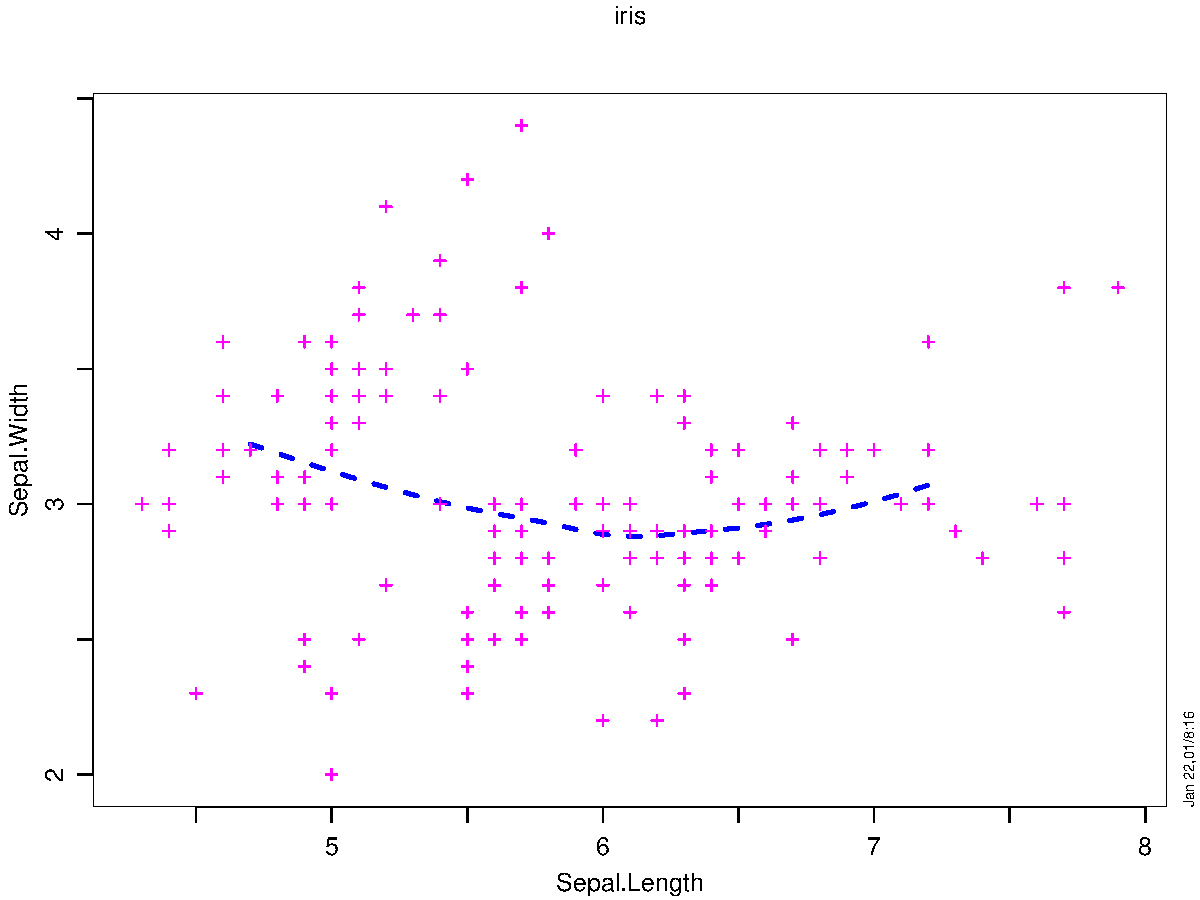
\includegraphics[width=\maxwidth]{figure/ploptions-1} 
\begin{kframe}\begin{alltt}
\hlcom{## restore the old optios}
\hlkwd{ploptions}\hlstd{(}\hlkwc{list}\hlstd{=}\hlkwd{attr}\hlstd{(t.plopt,} \hlstr{"old"}\hlstd{))}
\end{alltt}
\end{kframe}
\end{knitrout}

There are some differences between the behavior of \T{ploptions} and \T{par}:
\begin{itemize}
\item 
The pl options are stored in a list \T{.ploptions} in the global
environment and are therefore not erased when leaving the R session with
saving the workspace (\T{q(save="yes")}).
\item
There is a list \T{ploptionsDefault} in the package. It collects the
package's default settings and is used as a backup if some components should
not be contained in \T{.ploptions}.
\item
Both of these lists can be overriden by objects with the same name
that appear earlier in the search list than the \T{plgraphics} package.
\item
The value returned by \T{ploptions} is the entire, modified list of 
pl options. The old values are stored in the attribute \T{attr( ,"old")}
to be used for restoring them, see above.
\end{itemize}


\Remark
The concept of the ploptions list is a version of a more general idea, 
suggesting that the default values of any ``high level'' R function should 
have an associated list of default arguments, which is not contained in 
the function definition, but stored separately. 
This would allow the user more generally to specify his own style by 
changing these defaults and storing them in a kind of style file to be 
loaded at the start of each session. 
Here, there is only one list because the various pl functions need the 
same graphical elements.

Thus, a graphical element like a plotting character is generally searched 
in
\begin{enumerate}
\item 
  the argument list of the calling function,
\item
  the \T{ploptions} argument of the calling function,
\item
  the \T{.ploptions} list in the global environment or in the \T{search()} list,
\item
  the list \T{ploptionsDefault} in the package \T{plgraphics}
  or in an environment hiding it.
  %% same as .ploptions!
\end{enumerate}

The components of these lists include
\begin{itemize}
\item 
  \T{colors}, the palette of colors to be used;
\item
  \T{linewidth}, the linewidths used for the different line types.
  If the line types are shown with the same \T{lwd}, they are perceived
  with different intensity. \T{linewidth} intends to compensate this effect.
\item
  \T{cex}, a factor applied to the current value of \T{par("cex")} to
  determine the general character expansion used by the pl functions.
\item
  \T{cex.pch}, the median character expansion.
  The default is the function \T{cexSize}, with argument \T{n}, defined as
  \T{min(1.5/log10(n), 2)}, that is called when the number \T{n} of
  observations is available. Alternatively, a fixed scalar can be given.
\item
  a group of basic components:
  \T{pch, cex, cex.pch, cex.plab, lty, lwd, col}.\\
  \T{cex} is a factor which will be applied to \T{cex.pch} above for
  showing points by a single symbol (\T{pch}),\\
  \T{cex.plab} is an additional factor applied for the points that
  are shown by \T{plab}.
\item
  a group of compnents named \T{group} (\T{group.pch, ...}).
  They characterize how different groups will be displayed.
  Thus, \T{group.pch} should be a vector defining the plotting symbol
  for the first, second, ... group (when there are groups in the data).
\item
  a group named \T{variables}, 
  defining the elements to be used when different variables should be
  distinguishable;
\item
  \T{censored.pch} and \T{censored.cex} used to show censored observations;
\item
  \T{mar, oma, mgp, thickintervals}, specifying the number of lines in the
  figure's margins and outer margins, the ``margin parameters'' as in
  \T{par}, and the targeted number of tick intervals for axis labelling.
  The latter usually consists of 2 numbers, specifying the number of
  intervals for all ticks and for labelled ones, respectively. 
\item
  \T{stamp}, logical value determining if a stamp should be added in the
  bottom right corner of each plotting page;
\item
  a group \T{innerrange}, determining if and how an inner plotting range
  should be used and generated;
\item
  \T{plext}: percentage by which the range of the data should be
  extended unless an inner range is active (in which case the extension 
  is determined by \T{innerrange.ext}), and\\
  \T{plextext}: further extension to allow for large symbols near the 
  limits of the plotting range;
\item
  \T{markextremes} sets the proportion of extreme points that are shown 
  with labels to help identify them.
  If set to \code{TRUE}, the proportion depends on the number \T{n} of
  observations through \code{ceiling(sqrt(n)/2)/n}.
\item
  \T{title.cex} determines the character expansion of the plot title.
  By default, it adapts to the length of the title.
  For long titles, it will however never be smaller than
  \T{title.cexmin}. 
  If \T{title.cex} has 2 elements, the second refers to the subtitle.
\item
  a group \T{grid}. If \code{grid} is a list of two vectors,
  it contains the values where vertical and horizontal thin lines are drawn.
  If it is \T{TRUE}, the gridlines correspond to the tickmarks of the
  two axes.
  \T{grid.lty, grid.lwd, grid.col} set the respective
  properties for the gridlines.
\item
  a group \T{zeroline}, which is analogous to \T{grid}, but the
  default of \T{zeroline} is \T{TRUE}, which leads to using 
  0 for numerical variables and none for factors. 
  The properties are independent of those for \T{grid};
\item
  a group \T{refline}, where the component \T{refline} can be logical 
  or \T{==2},
  the latter indicating the a band should also be shown if available.
  Alternatively, \T{refline} can be a vector of length 2, which will be
  interpreted as intercept and slope of a straight line, or be
  a function that yields such a vector and takes as the first two 
  arguments \T{x} and \T{y} or a first argument named formula which 
  will be set to \T{y$\sim$x}.
  The properties \T{lty, lwd, col} to be used in \T{plrefline}
  are again defined as above;
\item
  a group \T{smooth}, containing items needed for generating and drawing
  smooth lines;
  \label{options.smooth}
%%- \item
%%-   a group \T{smooth}. If \T{smooth} is \T{TRUE}, a smoothing function 
%%-   with default \Hneed{80mm} \T{ploptions("smooth.function")} 
%%-   is called to calculate a
%%-   smooth line and show it according toe the \T{smoothline} properties;
\item
  a group \T{bar} needed to show reference values for levels of factors
  used as input variables in regression diagnostic plots;
\item
  \T{factor.show} indicates the way in which plots with factors are shown,
  presently only if one of the two variables (x or y) is a factor and the
  other, quantitative. Then, the factor can be jittered and then used
  as a quantitative variable, or a box plot or a ``multibox plot'' can be 
  chosen.
\item
  \T{jitter}: logical indicating if factors should be shown with jittering.
  A named vector may be given that defines the jittering for each
  variable.\\ 
  \T{jitter.factor} is the jittering factor used, see \T{?jitter}.
\item
  \T{condprobrange} is used to determine which bars should be shown
  in the case of censored data.
\item
  \T{functionxvalues} contains the number of argument values for which 
  a smooth function or fitting component is evaluated in diagnostic plots.
\item
  \T{leveragelimit} determines the range used for leverage values
  when plotting residuals against leverages.
\item
  A group \T{plcond} controlling features within the function \T{plcond}.
\end{itemize}

If these options modify any setting of R's \T{par} list and they are 
set as arguments to high level pl functions 
(\T{plyx, plmatrix, plmboxes, plregr, plresx}), as well as 
\T{plframe} and \T{plaxis},
they are restored after leaving the function (please report failures!).
When \T{plmframes} is called by the user, the information to restore 
the old settings is contained in its (invisible) value.
Thus, 
\begin{knitrout}
\definecolor{shadecolor}{rgb}{0.969, 0.969, 0.969}\color{fgcolor}\begin{kframe}
\begin{alltt}
\hlstd{op} \hlkwb{<-} \hlkwd{plmframes}\hlstd{(}\hlnum{1}\hlstd{,}\hlnum{3}\hlstd{)}
\hlcom{## plyx(Sepal.Width~Sepal.Length, data=iris, group=Species, mar=c(3,1,3,0))}
\hlkwd{par}\hlstd{(}\hlkwd{attr}\hlstd{(op,} \hlstr{"oldpar"}\hlstd{))}
\hlkwd{par}\hlstd{(}\hlstr{"mfg"}\hlstd{)}
\end{alltt}
\begin{verbatim}
## [1] 1 1 1 1
\end{verbatim}
\end{kframe}
\end{knitrout}
will restore the old settings. Here, we have commented out the plotting
statement to save space.

The options that are finally used in high level pl displays are saved 
in the list \T{.plargs} in the global environment as
\T{.plargs\$ploptions}.
This allows for re-using the same settings and may help debugging when
displays do not show what was desired.

%% ---------------------------------
\subsection{Graphical metadata, attributes of variables used for plotting}
%%pl.control, pldata, plargs
\label{plproperties}
Pl graphics rely on generating and maintaining metadata that guide the
details of creating the plots. 
%% They are described in the following paragraphs. 
They are stored as an enriched dataset that contains the variables needed
for the displays called \T{pldata}. We first describe them and then show
how \T{pldata} is generated and made available.

\Tit{Progperties of observations.}
The first type of such properties relates to the observations and includes
the plotting symbol, color and size for each of them.
These specifications are
\begin{itemize}
\item 
  \T{pch}: plotting symbol (character);
\item
  \T{plab}: plotting label, an extension of \T{pch} to more than one symbol,
  often used to identify observations;
\item
  \T{psize}: plotting size, scaled by the pl option \T{cex};
\item
  \T{pcol}: color of the symbol.
\end{itemize}
These elements are stored in \T{pldata} as columns with names
\T{(pch)}, \T{(plab)}, \T{(psize)}, \T{(pcol)}.
They are specified by the user usually by setting the corresponding
arguments \T{pch, plab, psize, pcol} in high level pl functions.
These arguments are not listed explicitly in the help files of 
the high level functions. 
Instead, these functions call \T{pl.control} to set them.
Alternatively, they may already be contained in the dataset given by the 
argument \T{data}.
\begin{knitrout}
\definecolor{shadecolor}{rgb}{0.969, 0.969, 0.969}\color{fgcolor}\begin{kframe}
\begin{alltt}
\hlkwd{plyx}\hlstd{(Sepal.Width}\hlopt{~}\hlstd{Sepal.Length,} \hlkwc{data}\hlstd{=iris,}
     \hlkwc{pch}\hlstd{=Species,} \hlkwc{psize}\hlstd{=Petal.Length,} \hlkwc{pcol}\hlstd{=Species)}
\end{alltt}
\end{kframe}
\includegraphics[width=\maxwidth]{figure/plyx_pattr-1} 
\begin{kframe}\begin{alltt}
\hlkwd{table}\hlstd{(.plargs}\hlopt{$}\hlstd{pldata[,}\hlstr{".pch."}\hlstd{])}
\end{alltt}
\begin{verbatim}
## 
##  1  2  3 
## 50 50 50
\end{verbatim}
\end{kframe}
\end{knitrout}
As the last statement shows, the \T{pldata} dataset is available after
calling the plotting function as a component of the list \T{.plargs}.

\Tit{Properties of variables.}
A second type of properties determines how variables should be displayed.
These are
\begin{itemize}
\item
  \T{varname} and \T{varlabel}: variable name and label --  
  to be used for labelling the axis on which the variable is shown --, 
  typically identical to the name of the variable
  in the data.frame it comes from;
\item
  \T{ticksat}: the values for which tick marks will be shown in plots.
  This item may carry an attribute \T{small} that leads to an additional
  set of smaller tickmarks;
\item
  \T{ticklabelsat} the possibly tick labels \T{ticklabels}:
  positions of labels to indicate values of the variable, and the lablels
  themselves;
\item
  \T{innerrange, plrange}: inner and outer plotting range;
\item
  \T{innerrange.ext}: extension used to calculate \T{plrange}
  from \T{innerrange}, if the latter does not cover all points;
\item 
  \T{nouter}: the number of points modified at each end of the inner range;
\item
  \T{numvalues}: numerical values to represent the given data values in
  case these are not numeric or for other reasons, see \T{plscale} and
  \T{gendateaxis} below;
\item
  \T{plcoord}: coordinates, possibly different from the variable's data
  values, typically when an inner plotting range or jittering is active;
\item
  \T{pch, lty, col}: plotting symbol, line type and color to be used 
  if multiple y's are shown in a plot.
\end{itemize}
These elements are stored as attributes of the variables,
e.g., \T{attr(var, "thicksat")}.
They can be set (or generated by the function \T{genvarattributes} and 
then modified) before calling the high level pl function.
Those that are needed and have not been stored beforehand will be 
generated by \T{pl.control} when calling such a function.
\begin{knitrout}
\definecolor{shadecolor}{rgb}{0.969, 0.969, 0.969}\color{fgcolor}\begin{kframe}
\begin{alltt}
\hlstd{dd} \hlkwb{<-} \hlstd{iris} \hlcom{## (avoid a modified version of  iris  in .GlobalEnv)}
\hlkwd{attr}\hlstd{(dd}\hlopt{$}\hlstd{Sepal.Length,} \hlstr{"ticksat"}\hlstd{)} \hlkwb{<-} \hlkwd{structure}\hlstd{(}\hlkwd{seq}\hlstd{(}\hlnum{4}\hlstd{,} \hlnum{8}\hlstd{,} \hlnum{1}\hlstd{),} \hlkwc{small}\hlstd{=}\hlkwd{seq}\hlstd{(}\hlnum{4}\hlstd{,}\hlnum{8}\hlstd{,}\hlnum{0.2}\hlstd{))}

\hlkwd{plyx}\hlstd{(Sepal.Width}\hlopt{~}\hlstd{Sepal.Length,} \hlkwc{data}\hlstd{=dd,}
     \hlkwc{grid}\hlstd{=}\hlkwd{list}\hlstd{(}\hlkwc{Sepal.Length}\hlstd{=}\hlkwd{seq}\hlstd{(}\hlnum{4}\hlstd{,}\hlnum{8}\hlstd{,}\hlnum{0.5}\hlstd{)))}
\end{alltt}
\end{kframe}
\includegraphics[width=\maxwidth]{figure/varattributes-1} 

\end{knitrout}

\Tit{\T{pl.control}.}
High level pl functions call the function \T{pl.control} first.
It generates the ``plotting dataset'' \T{pldata}, which
collects data dependent information needed for plotting in an enriched,
standardized form. 
It also takes any futher arguments to be passed on to \T{ploptions}.
The result is stored as \T{.plargs} in the global environment.
This allows for inspection of the plotting data
\T{.plargs\$pldata} and the active \T{ploptions} (\T{.plargs\$ploptions})
and thereby helps debugging.

\Tit{Plot scale.}
Showing a variable with a ``plot scale'', like ``log scale'', means
to transform the values with a given function (\T{log}), storing them
in the attribute \T{numvalues}, and setting 
\T{ticksat, ticklabelsat} and \T{ticklabels} corresponding to ``pretty''
values of the original scale.
The function that generates these attributes is \T{plscale}.
It can be called explicitly in order to fix the scale as a property
of the variable in the dataset it comes from, or implicitly by 
setting the argument \T{plscale} when calling a high level function,
see \ref{intro.plscale}.
\begin{knitrout}
\definecolor{shadecolor}{rgb}{0.969, 0.969, 0.969}\color{fgcolor}\begin{kframe}
\begin{alltt}
  \hlstd{dd} \hlkwb{<-} \hlstd{d.babysurvGr}
  \hlkwd{plyx}\hlstd{(}\hlkwd{I}\hlstd{(}\hlnum{100}\hlopt{*}\hlstd{Survival.1}\hlopt{/}\hlstd{n)} \hlopt{~} \hlstd{Weight,} \hlkwc{data}\hlstd{=d.babysurvGr,} \hlkwc{plscale}\hlstd{=}\hlkwd{c}\hlstd{(}\hlstr{"log"}\hlstd{,}\hlstr{"asinp"}\hlstd{))}
\end{alltt}
\end{kframe}
\includegraphics[width=\maxwidth]{figure/plscale-1} 
\begin{kframe}\begin{alltt}
  \hlcom{## or, in order to fix the plotting scale for further use}
  \hlstd{t.survp} \hlkwb{<-} \hlkwd{with}\hlstd{(dd,} \hlnum{100}\hlopt{*}\hlstd{Survival.1}\hlopt{/}\hlstd{n)}
  \hlstd{dd}\hlopt{$}\hlstd{SurvPerc} \hlkwb{<-} \hlkwd{plscale}\hlstd{(t.survp,} \hlstr{"asinp"}\hlstd{)}
  \hlstd{dd}\hlopt{$}\hlstd{Weight} \hlkwb{<-} \hlkwd{plscale}\hlstd{(dd}\hlopt{$}\hlstd{Weight,} \hlstr{"log"}\hlstd{)}
  \hlkwd{attr}\hlstd{(dd}\hlopt{$}\hlstd{Weight,} \hlstr{"ticklabels"}\hlstd{)}
\end{alltt}
\begin{verbatim}
## [1] "600"  "700"  "800"  "1000" "1200" "1500"
\end{verbatim}
\begin{alltt}
  \hlkwd{str}\hlstd{(dd}\hlopt{$}\hlstd{SurvPerc)}
\end{alltt}
\begin{verbatim}
##  num [1:10] 0 14.3 33.3 36.4 71.9 ...
##  - attr(*, "numvalues")= num [1:10] 0 0.247 0.392 0.412 0.644 ...
##  - attr(*, "ticksat")= num [1:6] 0 0.205 0.295 0.436 0.564 ...
##  - attr(*, "ticklabels")= chr [1:6] "0" "10" "20" "40" ...
##  - attr(*, "plscale")= chr "asinp"
\end{verbatim}
\begin{alltt}
  \hlcom{## or  dd <- genvarattributes(dd, plscale=c(Weight="log",SurvPerc="asinp"))}
  \hlcom{## plyx(SurvPerc~Weight, data=dd) ## now produces the same plot as above}
\end{alltt}
\end{kframe}
\end{knitrout}

\Tit{Date variable.}\label{options.dateaxis}
Similarly, the function \T{gendateaxis} provides nice tick values and labels 
for variables expressing a date or time. 
The function \T{gendate} helps to generate such a date. 
If a variable inherits from class \T{Date} or \T{times}, it will be shown
automatically in this way.

\subsection{Graphical parameters inside and outside high level pl functions}
The high level pl functions set graphical parameters (by calling \T{par}) 
according to their needs and often set pl options. 
When they end, they reset the \T{par} parameters to the previous values
unless the argument \T{keeppar} is \T{TRUE}.
Since quite often, the parameters determining the width of the plot margins are
changed, subsequent calls to low level R functions would not work properly,
that is, points within the plotting area as well as elements put to the 
margin by \T{mtext(...)} would be wrongly positioned.
As an alternative to setting \T{keeppar=TRUE}, the function \T{plpar}
can be called to set the ``margin parameters'' \T{mar, oma, mgp, cex}
to the values used in the last call to a high level pl function.
These are available from \T{.plargs\$ploptions} 
(unless \T{assign} was \T{FALSE} in this call).

\begin{knitrout}
\definecolor{shadecolor}{rgb}{0.969, 0.969, 0.969}\color{fgcolor}\begin{kframe}
\begin{alltt}
\hlkwd{plmframes}\hlstd{(}\hlnum{1}\hlstd{,}\hlnum{2}\hlstd{)}

\hlkwd{par}\hlstd{(}\hlkwc{mar}\hlstd{=}\hlkwd{c}\hlstd{(}\hlnum{2}\hlstd{,}\hlnum{2}\hlstd{,}\hlnum{5}\hlstd{,}\hlnum{2}\hlstd{))}
\hlkwd{plyx}\hlstd{(Sepal.Width}\hlopt{~}\hlstd{Sepal.Length,} \hlkwc{data}\hlstd{=iris)} \hlcom{## margins according to ploptions}
\hlkwd{par}\hlstd{(}\hlstr{"mar"}\hlstd{)} \hlcom{## paramteres have been recovered}
\end{alltt}
\begin{verbatim}
## [1] 2 2 5 2
\end{verbatim}
\begin{alltt}
\hlkwd{mtext}\hlstd{(}\hlstr{"wrong place for text"}\hlstd{,}\hlnum{3}\hlstd{,}\hlnum{1}\hlstd{,} \hlkwc{col}\hlstd{=}\hlstr{"red"}\hlstd{)}  \hlcom{## margins not appropriate for active plot}
\hlstd{t.usr} \hlkwb{<-} \hlkwd{par}\hlstd{(}\hlstr{"usr"}\hlstd{)}
\hlkwd{points}\hlstd{(t.usr[}\hlnum{2}\hlstd{],t.usr[}\hlnum{4}\hlstd{],} \hlkwc{pch}\hlstd{=}\hlstr{"X"}\hlstd{,} \hlkwc{col}\hlstd{=}\hlstr{"red"}\hlstd{)}
\hlkwd{plpoints}\hlstd{(t.usr[}\hlnum{2}\hlstd{],t.usr[}\hlnum{4}\hlstd{],} \hlkwc{pch}\hlstd{=}\hlstr{"+"}\hlstd{,} \hlkwc{col}\hlstd{=}\hlstr{"blue"}\hlstd{)}
\end{alltt}
\begin{verbatim}
## NULL
\end{verbatim}
\begin{alltt}
\hlstd{t.plo} \hlkwb{<-} \hlkwd{plpar}\hlstd{()} \hlcom{## get margin parameters from .plargs }
  \hlcom{## generated by the last pl graphics call}
\hlkwd{par}\hlstd{(}\hlstr{"mar"}\hlstd{)}
\end{alltt}
\begin{verbatim}
## [1] 3.1 3.1 3.1 1.1
\end{verbatim}
\begin{alltt}
\hlkwd{mtext}\hlstd{(}\hlstr{"here is the right place"}\hlstd{,}\hlnum{3}\hlstd{,}\hlnum{1}\hlstd{,} \hlkwc{col}\hlstd{=}\hlstr{"blue"}\hlstd{)}
\hlkwd{points}\hlstd{(t.usr[}\hlnum{2}\hlstd{],t.usr[}\hlnum{4}\hlstd{],} \hlkwc{pch}\hlstd{=}\hlstr{"O"}\hlstd{,} \hlkwc{col}\hlstd{=}\hlstr{"blue"}\hlstd{)}

\hlkwd{par}\hlstd{(}\hlkwd{attr}\hlstd{(t.plo,} \hlstr{"oldpar"}\hlstd{))}  \hlcom{## restores old 'margin parameters' }
\hlkwd{par}\hlstd{(}\hlstr{"mar"}\hlstd{)}
\end{alltt}
\begin{verbatim}
## [1] 2 2 5 2
\end{verbatim}
\begin{alltt}
\hlkwd{plyx}\hlstd{(Sepal.Width}\hlopt{~}\hlstd{Sepal.Length,} \hlkwc{data}\hlstd{=iris,} \hlkwc{keeppar}\hlstd{=}\hlnum{TRUE}\hlstd{)}
\hlkwd{par}\hlstd{(}\hlstr{"mar"}\hlstd{)}
\end{alltt}
\begin{verbatim}
## [1] 3.1 3.1 3.1 1.1
\end{verbatim}
\begin{alltt}
\hlkwd{mtext}\hlstd{(}\hlstr{"this goes to the right place, too"}\hlstd{,}\hlnum{3}\hlstd{,}\hlnum{1}\hlstd{)}
\end{alltt}
\end{kframe}
\includegraphics[width=\maxwidth]{figure/marginpars-1} 

\end{knitrout}

The low level pl functions to be presented next avoid this problem.
However, if you want to use these for adding to a figure started with
a standard plotting function (and you have different margin parameters
from those in \T{.ploptions}), then you need to set \T{setpar=FALSE}
in their call.
\begin{knitrout}
\definecolor{shadecolor}{rgb}{0.969, 0.969, 0.969}\color{fgcolor}\begin{kframe}
\begin{alltt}
\hlkwd{par}\hlstd{(}\hlkwc{mar}\hlstd{=}\hlkwd{c}\hlstd{(}\hlnum{2}\hlstd{,}\hlnum{2}\hlstd{,}\hlnum{5}\hlstd{,}\hlnum{2}\hlstd{))}
\hlkwd{plot}\hlstd{(}\hlnum{1}\hlopt{:}\hlnum{10}\hlstd{)}
\hlkwd{plpoints}\hlstd{(}\hlnum{8}\hlstd{,}\hlnum{9}\hlstd{,} \hlkwc{col}\hlstd{=}\hlstr{"red"}\hlstd{)} \hlcom{## wrong}
\end{alltt}
\begin{verbatim}
## NULL
\end{verbatim}
\begin{alltt}
\hlkwd{plpoints}\hlstd{(}\hlnum{8}\hlstd{,}\hlnum{9}\hlstd{,} \hlkwc{col}\hlstd{=}\hlstr{"blue"}\hlstd{,} \hlkwc{setpar}\hlstd{=}\hlnum{FALSE}\hlstd{)} \hlcom{## correct}
\end{alltt}
\end{kframe}
\includegraphics[width=\maxwidth]{figure/parproblem-1} 
\begin{kframe}\begin{verbatim}
## NULL
\end{verbatim}
\end{kframe}
\end{knitrout}
%% -----------------------------------------------------------
\section{Low level graphics}

Like in basic R, there are ``low level'' graphical functions that
add to an existing plot, whereas ``high level'' functions are designed to 
generate a full plot. Low level plotting functions include:

\begin{itemize}
\item 
  \T{plframe} generates a new frame, frames the inner and outer plotting
  ranges and draws gridlines and axes, the latter by calling \T{plaxis}. 
\item
  \T{plaxis} draws an axis based on the attributes of the variable given as
  the second argument.   
\item
\T{plpoints} draws points and lines. \\
  In the simplest case, this function places the plotting symbol at the
  given coordinates. As the basic \T{points} function, it draws lines if 
  the argument \T{type} is set to \T{"l"} or \T{"b"}, and the argument
  \T{pch} (or the column \T{".pch."} in \T{plargs\$pldata}) can provide
  different plotting symbols for the different points.\\

  \T{plpoints} also includes the capabilities of \T{text}: 
  If the argument \T{plab} 
  is set (or \T{plargs\$pladata} contains a column named \T{".plab."}),
  it should be a character vector and is reproduced at the (x,y) locations,
  Values \T{NA} or \T{""} being replaced by the plotting symbol in \T{pch}.\\
  The size of the plotting symbols or strings is determined by
  \T{plargs\$pldata[,"psize"]} if available and by the ploptions
  \T{cex} and \T{cex.pch}.

  If one or both coordinate variables contain censored values (that is,
  if they inherit from the class \T{"Surv"}), the censored observations are
  shown by the appropriate symbol from \T{ploptions("censored.pch")} and 
  with paled color (according to \T{ploptions("censored.pale")}).
\item
  \T{plmark} can be used to mark extreme points by labels and leave the
  non-extreme ones to be shown by the plotting symbol.
\item
  \T{plsmooth} and \T{plsmoothline} generates a smooth line and draws it 
  in the plot, respectively.
\item
  \T{plrefline} adds reference lines (straight lines or curves) to a plot.
  It is used by \T{plregr} and \T{plresx}.
%%-   as a vector giving intercept and slope of a straight line.
%%-   or a function that returns this list, such as \T{lm};
\item
  \T{pltitle} adds a title. By default, the character size 
  (given by the ploption \T{"title.cex"} is descreased
  for long titles (\T{main} or \T{sub}) to fit it onto one line.
\item
  \T{pllimits} and \T{plcoord} determine inner plotting range 
  (see above) and the respective coordinates where the points outside of it
  will appear on the plot.
\item
  \T{stamp} adds a time stamp and, if available, a project and analysis
  step title to the right bottom corner of the plotting page.
  This is avoided by setting \T{ploptions(stamp=FALSE)}.
\end{itemize}

\Tit{\T{plpanel}} is a ``medium level'' function. It calls all of the above
functions.
The user can re-program this function to modify and expand the actions that
are taken, store the modified function, e.g. under \T{my.panel}
and then set %% \T{ploptions(panel=my.panel)}
the argument \T{panel = my.panel} in \T{plyx} and \T{plmatrix},
or change the ploption, \T{ploptions(panel=my.panel)}.

\Tit{Coordinates from last high level pl function.}
The low level functions that act on \T{x} and \T{y} coordinates can be used
with empty \T{x} and \T{y} arguments. They will then obtain these values
from \T{.plargs\$pldata}, which is generated and stored by high level 
pl functions and will thus reflect the coordinates that are likely the
bases of the current plot. 
The pl options are also recovered from \T{.plargs} (unless the argument
\T{ploptions} is specified in the call to the low level function).


\section{Auxiliary functions}
These functions do calculations needed for generating graphical elements
(like generating a smooth) or are useful additional functions,
like \T{showd}, which displays a kind of summary of data.
Let us start with the latter category.

\Tit{Displaying data by \T{showd}.}
This function is useful for inspecting a data set or another object, 
avoiding overwhelming output. 
If the number of rows or list components is larger than 4,
the first 3 of them and the last one are shown only.
For rows in data.frames or matrices, two of the rows between the forth and
the last one are also printed.

\Tit{Subset of a data.frame.}
The function \T{plsubset} extracts a subset of a data.frame in a similar way
as the \T{subset} function of plain R.
The essential enhancement is that it keeps the graphical metadata and 
adjusts it where necessary.

%% \T{dropdata}  braucht es das?
%%- There is an additional function \T{dropdata} which allows for dropping
%%- observations or variables based on their names.

\Tit{Counting \T{NA}'s.}
\T{sumNA} counts the number of \T{NA}'s in vectors, matrices, and lists, 
including data.frames. 
For numerical objects, infinite values are counted as \T{NA}'s 
(unless the argument \T{inf} is \T{FALSE}).

\Tit{Started logarithm.}
Variables that contain only positive numbers usually call for a 
log transformation according to the ``first aid transformation'' principle
of data analysis introduced by John Tukey.
If they also contain zeros, the \T{log} function turns them into \T{-Inf}.
This is rarely desirable. 
A common way to avoid it is to add 1 to the variable before taking logs.
This is unreasonable, since adding 1 has a very different effect on the
result, depending on the magnitude of the range of non-zero values of the
variable. At least, the constant should adapt to this magnitude.
Another solution of the problem is given by the rule that below some
value $c$, the function should be linear, with a smooth derivative in $c$.
%%
%%- \texttt{regr} includes a function \texttt{logst} that is based on the
%%- following ideas:
%%- \begin{itemize}
%%- \item 
%%- The modification should only affect the values for ``small'' arguments.
%%- \item
%%- What is ``small'' should be determined in connection with the non-zero 
%%- values of the original variable, since it should behave well (be
%%- equivariant) with respect to a change in the ``unit of measurement''.
%%- \item
%%- The function must remain monotone, and it should remain (weakly) convex.
%%- \end{itemize}
This is implemented in the function \T{logst}, defining the value $c$
as a function of the quartiles of the non-zero values.

%%- The function \texttt{logst} implements these criteria in the following way: 
%%- The shape is determined by a threshold $c$ at which -- coming from above --
%%- the log function switches to a linear function with the same slope at this
%%- point. This is obtained by
To be precise, \T{logst} is defined as
$$
%%  g(x) = 
         \left\{\begin{array}{ll}\log_{10}(x) & \mbox{if\ \ } x\ge c\\
         \log_{10}(c) - (c-x)/(c\log(10)) & \mbox{if\ \ } x< c
         \end{array}\right.
\;.$$
The threshold $c$ is set to
$ c = q_1^{1+r}/q_3^r$, where $q_1$ and $q_3$ are the quartiles of the 
positive data and $r$ is a tuning constant. 
The default of $r$ is 1 and leads to an expected
percentage of about 2\% of the data below $c$ for log-normal data.
It is certainly useful to inspect a graph of the function, as drawn in 
\texttt{example(logst)}.

The use of \T{logst} in regression will cause problems when calculating
predicted values for new data, since its result depends on the whole
dataset through the determination of $c$ by default. 
Therefore, $c$ can be given to \T{logst} by the argument \T{threshold}.

Other auxiliary functions include
\begin{itemize}
\item
  \T{getvariables} gets the variables contained in a formula.
\item 
  \T{clipat}, drops data outside a range or recplaces them with \T{NA}
  or a suitable value.
\item
  \T{warn} summarizes warnings, thus avoiding endless repetitions of the
  same warning.
\end{itemize}

\Tit{Plotting properties.}
Auxiliary functions used for getting plotting properties are
\begin{itemize}
\item
  \T{gensmooth}, the wrapper function for getting smooths.
  It in turn calls \T{smoothRegr} by default.
\item 
  \T{robrange} determines a robust range of data to be used as inner
  plotting range.
\item
  \T{simresiduals} simulates residuals used for generating additional
  smooths to which the actual one can be compared.
\item
  \T{colorpale} determines a paled version of a color.
\end{itemize}


%%- \subsection{Multiple Frames}
%%- Function \T{plmframes} splits the screen by calling \T{par(mfrow=...)}.
%%- It adds flexibility and sets other defaults for margin widths and the like. 
%%- 

%% =========================================================================
\section{Details}

%%- \subsection{plargs, ploptions, default values} 
%%- (if needed, see above)
%%- 
%%- \Tit{Default values.}
%%- \T{i.def}
%%- \T{i.getploption} and \T{i.getplopt}
%%- 
%%- Some arguments to low level pl functions need to be set by changing
%%- the \T{ploptions} argument.
%%- Example:
%%- 
%%- residuals in plargs are data.frame
%%- 
%%- variable colors, ... stored in pdata
%%- generated in pl.control avoiding elements already in use 
\subsection{Palette}
Even though the palette that is active in the global environment is not
affected, the pl functions use an implicit palette given by 
\T{ploptions("colors")}. By default, the list is
\begin{knitrout}
\definecolor{shadecolor}{rgb}{0.969, 0.969, 0.969}\color{fgcolor}\begin{kframe}
\begin{alltt}
\hlstd{ploptionsDefault}\hlopt{$}\hlstd{colors}
\end{alltt}
\begin{verbatim}
##  [1] "black"        "red"          "blue"         "darkgreen"   
##  [5] "orange"       "purple"       "deepskyblue2" "green3"      
##  [9] "coral4"       "pink3"        "aquamarine3"  "brown2"
\end{verbatim}
\end{kframe}
\end{knitrout}
The selection of these colors has been driven by the following ideas:
\begin{itemize}
\item 
  The first few should be readily distinguishable and reflect a common 
  sequence: after the default ``black'', the most salient one is red,
  followed by blue, then ``darkgreen'' because ``green'' is lighter than
  the foregoing, and finally ``orange''.
\item
  The first colors should be simply named. If the user explicitly sets one
  of them, e.g., by \T{attr(data\$var, "col") \Gets\ "red"}, the pl
  functions have a chance to avoid them when making default decisions.
\item
  After the first group of 4 alternative colors, another group of 4 follows.
  It is a modification of the first group. The third group is incomplete as
  no blueish color could be found that would be distint enough from the 
  foregoing colers.
\end{itemize}

\subsection{Point labelling and plotting character}
The properties of the symbols displaying observations are set by the
following rules.
\begin{enumerate}
\item 
  If they are specified by the respective argument to high level \T{pl} 
  function (and evaluated by \T{pl.control}), this has priority
  (excemption, see 2.).
\item
  In the case of multiple $y$s, colors are determined primarily by 
  the argument \T{vcol} of the high level \T{pl} function, 
  scondarily by the \T{vcol} attribute of the variables. 
  Thirdly, \T{ploptions("variables.col")} is used,
  avoiding colors that are already specified for some variables by the
  foregoing steps (see \T{i.getvarattribute}, called by 
  \T{genvarattributes} in 
  \T{pl.control}.)\\
  If \T{pch} is not determined otherwise (argument, see 1., or group,
  see 3.) it is set in the same way.\\
  For plots of type \T{"l"} or \T{"b"}, the line type \T{lty} is determined 
  in the same way as the color.
\item
  If there is grouping and only a single $y$, the group determines \T{pch}
  and its color by the \T{group} components of \T{ploptions} unless set
  by 1. above.
\item
  In other cases, the \T{default} group of \T{ploptions} is used.
\end{enumerate}

\subsection{Groups}

Pl functions may use a grouping of observations, defined by an argument
\T{group=...} in different ways.
\T{plyx} splits the observations accordingly and produces a panel for each
group.

Other types of groupings are:
\begin{itemize}
\item
  \ul{Smooth groups.} \
  The argument \T{smooth.group} allows for drawing a separate smooth line 
  for each group.
\item 
  \ul{Color.} \
  Groups get different colors by specifying \T{pcol}.
  If the value is a factor, it will be converted into 
  \T{ploptions("group.col")[as.numeric(pcol)]}.
  In order to give color by color names, make sure that \T{pcol} is
  a character variable.
\end{itemize}

\subsection{Axes, plotting ranges}

\Tit{Setting pl ranges.}
The regular and inner plotting ranges can be set by specifying
\T{plrange} and \T{innerrange} in the high level pl function 
by giving a named list of vectors of length 2.
Alternatively, a range can be specified for any variable in a dataset
by setting the attribute \T{attr(dd, "plrange")} or
\T{attr(dd, "innerrange")} or both.

Set the \T{innerrange} attribute by calling \T{genvarattributes}. 
Otherwise, you need to call also \T{plcoord} in order to have a conforming
\T{plcoord} attribute of the variable(s).

Note that the resulting \T{innerrange} may differ from the required 
inner range at the end(s) where no data are modified (\T{nouter==0}).

\Tit{Tick marks.}
The tick mark occur in three ``degrees'', the first one being labelled,
the second (called ``regular'') being only shown by a mark, the third, 
by a short mark.
(The lengths of the tick marks are determined by the ploption \T{ticklength}.)

\Tit{Gridlines, zeroline.}
If the ploption \T{grid} is \T{TRUE}, grid lines will be drawn at each (regular)
tick of both axes. 
Alternatively, the variable attribute \T{gridline} can be specified either 
directly or by \T{setvarattribute}
(The plotting properties \T{col, lty, lwd} are determined by the ploptions
\T{grid.col, grid.lty, grid.lwd}.)

Likewise, lines can be obtained by setting the variable attribute \T{zeroline}
and the respective options. By default, a zero line is drawn at 0 for
numerical variables.

\Tit{Axis label.}
The plotting routine (\T{plframe}) will look for an attribute \T{varlabel}.
If it is not available, the name of the variable will be used.

\subsection{Smooths}

Within the graphical functions, smooths are generated by calling 
\T{gensmooth}. It calls the function determined by
\T{options("smooth.function")}, which defaults to \T{smoothRegr}, and that
function calls basic R's \T{loess}.

The smoothing parameter, which in the default option is the \T{span}
argument of \T{loess}, depends on the number of observations by the function
\T{smoothpar} (unless set differently by the user).

%% ============================================== plreggr
\subsection{Standardized residuals}

\[
R^*_i=R_i\left/\left(\wh\sigma \sqrt{w_i} \sqrt{1-H_{ii}}\right)\right.
\]

Standardization ratio: 
$\T{stratio}_i=R^*_i/R_i$

\T{i.stres} calculates leverages, standardized residuals, and \T{strratio}
according to this formula.
For binary and Poisson models, ...

Cook's distance:
\[
  d_i\sups C=\frac{R_i^2\,H_{ii}}{p\wh\sigma^2\,(1-H_{ii})^2}
  =(1/p)\,R_i^{*2}\,H_{ii}/(1-H_{ii})
  \;,
\]
It is constant, $=d$, on the curve
\[
  R_i^{*2} = d\,p\,(1-H_{ii})/H_{ii}
\]
A rule suggests $d=4/(n-p)$ as a warning level.
Curves are drawn for $d=\T{cookdistlines}^2/(n-p)$.

\subsection{Modified methods for \T{residuals, fitted, predict}}
%
Some methods for the extractor functions \T{residuals, fitted, predict}
needed modifications and extensions.
For example, \T{type="link"} is needed for \T{polr} models.
The package contains a method \T{predict.regrpolr} which is used within the
package and provides the additional type, but is otherwise compatible with
\T{predict.polr} of the package \T{MASS}. It is exported.
Similarly, there are the methods
\T{fitted.regrpolr, residuals.regrpolr, residuals.regrsurvreg, 
  residuals.regrcoxph}.
Since a method for residuals is not available in the \T{MASS} package
for models fitted by \T{polr}, \Hneed{70mm}\T{residuals.regrpolr} is also
made available as \T{residuals.polr} and thereby provides the missing
method. 


\subsection{Missing values in residual analysis}
Model fitting functions in R support two different ways of dealing with
missing values. The default is determined by the value \T{na.omit}
of the argument \T{na.action}. 
This leads to residuals as extracted by the \T{residuals} function
and other analogous results that do not contain the observations with 
missing values in the data used for fitting.
As a consequence, they cannot be readily combined with variables from the
dataset. 
The alternative choice, \T{na.action=na.exclude}, corrects this flaw.
Vectors of residuals will contain \T{NA}s where appropriate and have 
the same length as the variables in the data.

The pl functions \T{plregr, plresx, plres2x} work with the extended
version. This is reflected in \T{.plargs\$pldata} and allows for
combining that data.frame with the original dataset.

\subsection{Documentation}
For a data analysis, it is often useful to save graphical displays in 
documents or on paper. In an extended data analysis, one can easily lose
control over the precise content of the different plots.
\T{plgraphics} provides some help for keeping track.
\begin{itemize}
\item 
  Every graphical display generated by a graphical function from the
  package gets a ``stamp'' in the lower right corner that indicates date
  and time of its creation and, if specified by the user before that 
  time point, a project title and a step name (by writing\\
  \T{ploptions(project=projecttitle, step=stepname)}).\\
  This stamp can of course be suppressed, e.g., for producing publication
  graphics: set \Hneed{40mm} \T{ploptions(stamp=FALSE)}.
\item
  Data sets may be documented by attaching two attributes, \T{tit} and 
  \T{doc} -- title and description --, which will be printed with
  numerical output if desired.
  Currently, this only works with the function \T{showd}.
  This feature is disabled by setting \T{ploptions(doc=FALSE)}.
\end{itemize}
\begin{knitrout}
\definecolor{shadecolor}{rgb}{0.969, 0.969, 0.969}\color{fgcolor}\begin{kframe}
\begin{alltt}
  \hlkwd{tit}\hlstd{(iris)} \hlkwb{<-} \hlstr{"Fisher's iris data"}
  \hlkwd{doc}\hlstd{(iris)} \hlkwb{<-} \hlstr{"The most famous statistical dataset ever"}
  \hlkwd{showd}\hlstd{(iris)}
\end{alltt}
\begin{verbatim}
## Fisher's iris data 
##    The most famous statistical dataset ever | The most famous statistical dataset ever | The most famous statistical dataset ever 
## dim:  150 5 
##     Sepal.Length Sepal.Width Petal.Length Petal.Width    Species
## 1            5.1         3.5          1.4         0.2     setosa
## 2            4.9         3.0          1.4         0.2     setosa
## 3            4.7         3.2          1.3         0.2     setosa
## ...                                                             
## 40           5.1         3.4          1.5         0.2     setosa
## 76           6.6         3.0          4.4         1.4 versicolor
## 113          6.8         3.0          5.5         2.1  virginica
## 150          5.9         3.0          5.1         1.8  virginica
\end{verbatim}
\end{kframe}
\end{knitrout}

%%- \section{Appendix}
%%- Additional functions and features.


%% =================================================================
\vspace{10mm}\noindent
{\small
\Tit{This is the end} of the story for the time being. I hope that you will
get into using \T{plgraphics} and have good success with your data analyses.
Feedback is highly appreciated.


Werner Stahel, \T{stahel at stat.math.ethz.ch}
}
\end{document}

%%% Local Variables: 
%%% mode: latex
%%% TeX-master: t
%%% End: 
